%%% describe all the experiments performed and their statistical analysis
\chapter{Results} % at least 10, maximum 40 pages

%%%%%%%%%%%%%%%%%%%%%%%%%%%%%%%%%%%%%%%%%%%%%%%%%%%%%%%%%%%%%%%%%%%%%%%%%%%%%%%%
\section{Characterization of Physicochemical Properties}
  \subsection{Stacking Potential}
    \subsubsection{Obtaining the Datasets}
      A total of $83500$ protein structure files were downloaded from the PDB, some of which also contained ligands. Similarly, $3032$ structures with protein and nucleic acid complexes where downloaded, with the presence of ligands in some of them. From these two datasets, $22786$ unique ligand IDs were observed. The CIF files for these ligands were also downloaded from the PDB.

    \subsubsection{Detecting Aromatic Groups in Ligands}
      The first method of detection (parsing the SMILES strings) found aromaticity in $18211$ ligands from the dataset, while the second method (simple topological examination of the structures) found aromatic groups in $19096$ ligand files. From these ligands, $388$ were detected only by the first method, while $1273$ were detected only by the second method, meaning that the detection methods disagreed in the case of $1661$ ligands (figure \ref{fig:results/stacking_detection}).

      \begin{figure}[H]
        \centering
        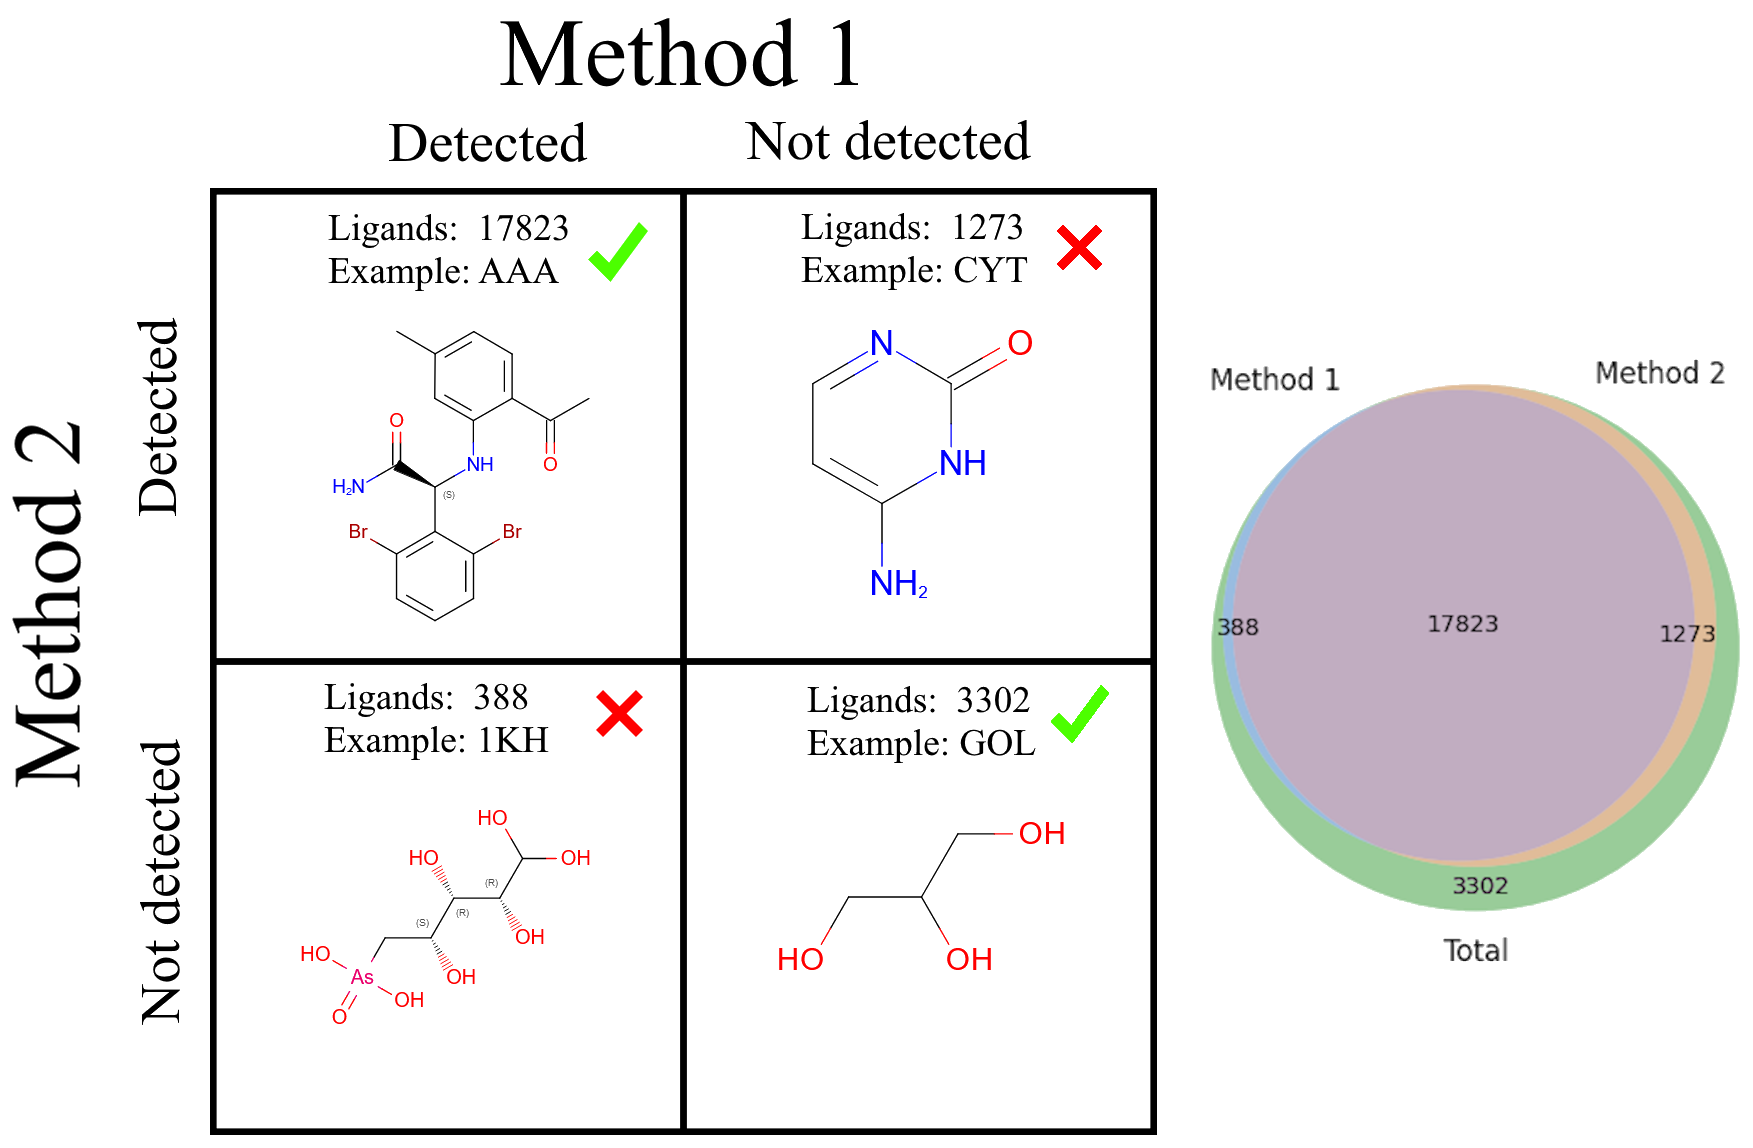
\includegraphics[width=0.8\textwidth]{figures/results/stacking_detection.png}
        \caption{\label{fig:results/stacking_detection} Example of ligands being tagged as aromatic or not by the two detection methods.}
      \end{figure}

      Some CIF files from the dataset had faulty SMILES strings (such as including the ligand name as a placeholder) or did not report correctly the aromaticity of the ligands. An example of the latter is the nucleic acid cytosine (CYT in figure \ref{fig:results/stacking_detection}), which is not properly identified as aromatic despite being a classic example of a biologically relevant aromatic group. This also was observed in uracil and other pyrimidines.

      The opposite situation also happened, where the SMILES string apparently contained aromatic atoms because lowercase symbols were found. However, this sometimes corresponded to unrelated heavy atoms. An example of this occurrence is the ligand 1KH in figure \ref{fig:results/stacking_detection}, whose arsenic atom is represented by "As" in the SMILES string, so the first method recognized the lowercase "s" as an aromatic sulfur. The second method however immediately discarded the ligand as it is acyclic.

      Some other instances with complex combinations of aromatic and non-aromatic rings (oftentimes connected by one or two atoms) presented problems for the second method, while being correctly reported in the first method. For these reasons, the $1661$ ambiguous ligands were manually inspected to clarify whether aromaticity was present or not. At the end of this process, $18298$ ligands (accounting for $80.3 \% $ of the original dataset) were found to present a combined total of $34807$ aromatic groups (on average, 1.9 aromatic groups per ligand).

    \subsubsection{Sampling of Aromatic Interactions}
      A total of $4843590$ interactions were sampled from the PDB dataset. The interaction datapoints were grouped according to their $\alpha$ and $\beta$ values. The average interaction distance for each group and their abundance in the dataset were inspected by means of a histogram (figure \ref{fig:results/stacking_sampling}.a).

      However, many of these datapoints could correspond to non-interacting aromatic groups in close proximity, which most likely occurs in \textbf{aminoacid-aminoacid} pairs. By filtering these out, $696676$ interactions remain, which accounts to $14 \%$ of those originally observed. The histogram of these datapoints is significantly less noisy, where seemingly most of the points are condensed in some specific regions of the $(\alpha, \beta)$ space (figure \ref{fig:results/stacking_sampling}.b).

      \begin{figure}[H]
        \centering
        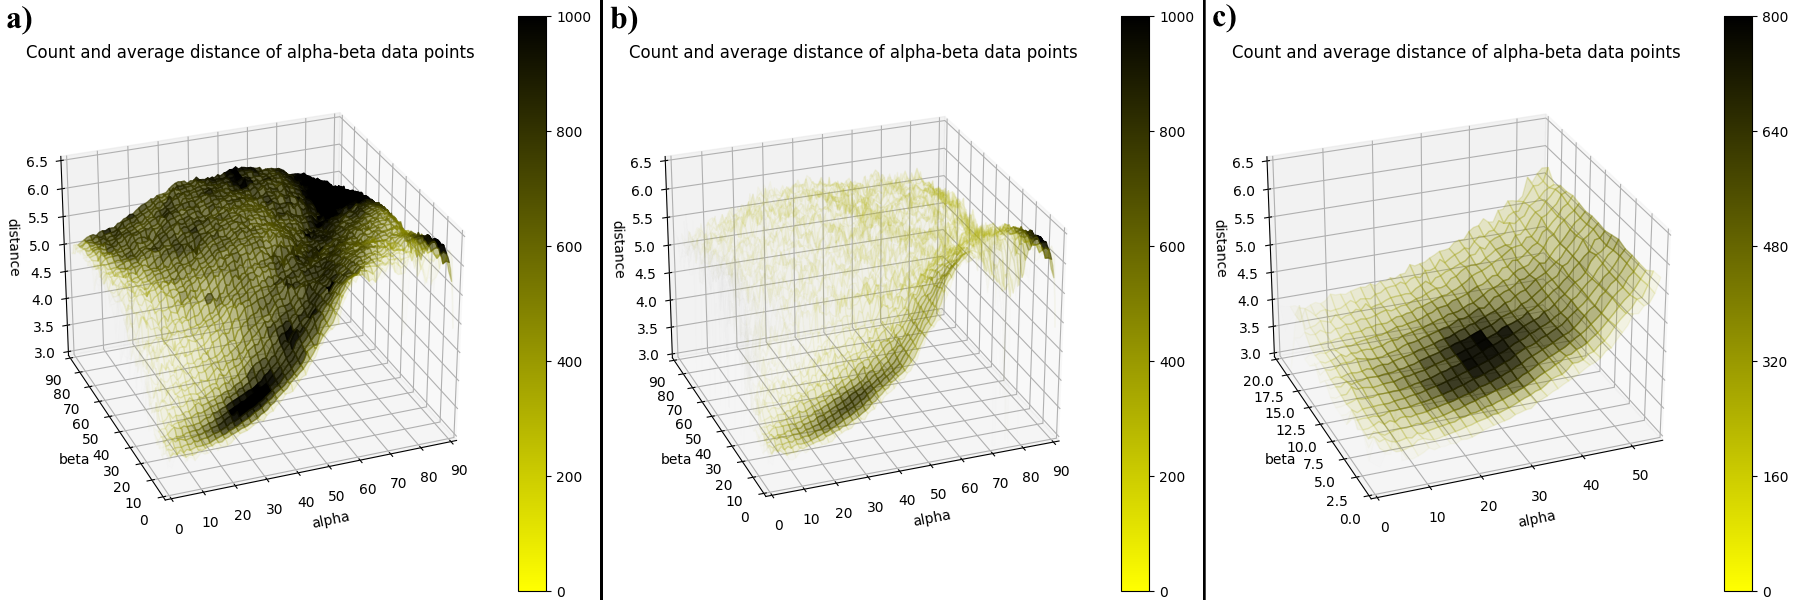
\includegraphics[width=1\textwidth]{figures/results/stacking_sampling.png}
        \caption{\label{fig:results/stacking_sampling} Interaction datapoints grouped by their $\alpha$ and $\beta$ values, with their average distance value reported as \textit{height} and amount of points for each group reported by \textit{color} (translucent yellow for few points, opaque black for many points). a) unfiltered interaction dataset, b) filtered dataset (no aminoacid-aminoacid interactions), c) filtered dataset focused on the range $\alpha \in [0,55], \beta \in [0,20]$.}
      \end{figure}

      A high density of interaction datapoints can be observed at low $\beta$, high $\alpha$ values and relatively long distances. This configuration mostly corresponds to base-pairing in PDB structures with nucleic acids, which can be further confirmed by filtering out \textbf{nucleic-nucleic} pairs (appendix figure \ref{fig:appx2/stacking_sampling}). Therefore, this region of points can be safely ignored.

      Another dense region of interaction datapoints can be observed spanning the range $\alpha \in [0,55], \beta \in [0,20]$. A total of $302651$ interactions are inside this range ($43 \%$ of the filtered datapoints). This range is also compatible with the theoretical configuration values of $\pi-\pi$ stacking potentials. Therefore, the empirical distribution of these values (figure \ref{fig:results/stacking_sampling}.c) will be used to define the model, suited to represent \textit{parallel-offset} stacking interactions specifically.

    \subsubsection{Model Definition}
      Some important observations must be noted before defining the stacking model:

      \begin{itemize}
        \item The histogram of the interactions of interest (figure \ref{fig:results/stacking_modelling}.a) reveals that varying the $\alpha$ value affects both the average distance of the points and their occurrence, while varying the $\beta$ value affects only the occurrence.
        \item The distance and the $\alpha$ value depend only on the position and normal vector of the aromatic group and the surrounding points in space, implying only three dimensions of space are needed for calculating them.
        \item The $\beta$ value depends on the normal vector of both the actual aromatic group and the hypothetical aromatic group which interacts with it. This means that the $\beta$ value requires a \textit{$\beta$ angle} dimension, which raises the same issue found when theorizing the hydrogen bond potential model.
      \end{itemize}

      Therefore, even if it would be ideal to use all three parameters when building the model, the model was defined to assume an ideal beta value of either $\beta \approx 0^{\circ}$ (theoretical) or $\beta \approx 7.5^{\circ}$ (empirical, figure \ref{fig:results/stacking_modelling}.a). The datapoints were then grouped considering only their $\alpha$, average distance and occurrence values observed in the histogram (figure \ref{fig:results/stacking_modelling}.b).

      \begin{figure}[H]
        \centering
        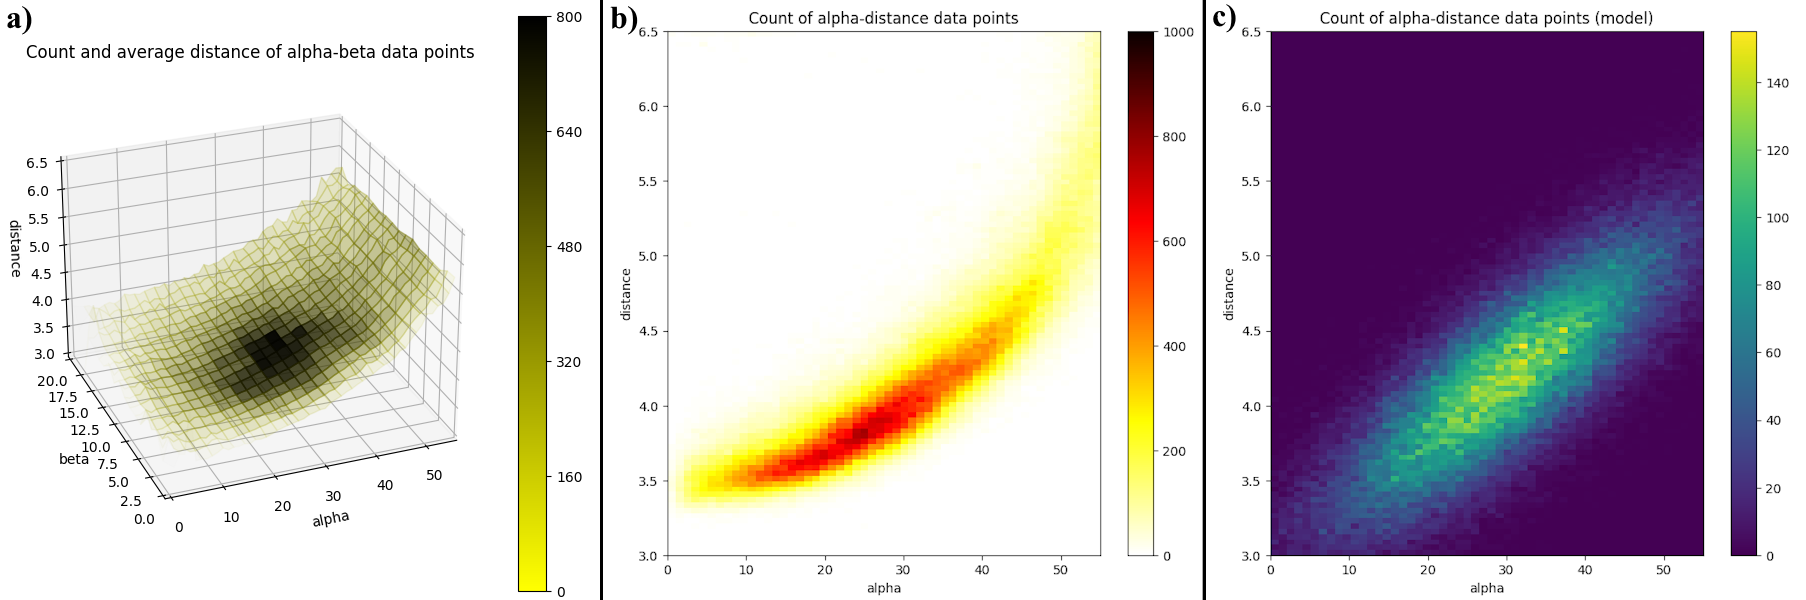
\includegraphics[width=1\textwidth]{figures/results/stacking_modelling.png}
        \caption{\label{fig:results/stacking_modelling} Empirical and modelled distribution of stacking interactions. a) same as figure \ref{fig:results/stacking_sampling}.c, b) same empirical datapoints, omitting the $\beta$ dimension, c) modelled datapoints.}
      \end{figure}

      The empirical distribution resembles a skewed normal distribution. Given that the distortion is not extreme, an approximation was introduced and the model was empirically determined to have the shape of a \textbf{2D normal distribution}, with dimensions being distance and $\alpha$ angle (instead of just distance, which is the case of hydrogen bonds and hydrophobicity). Note however that the domain of the function still consists of three spatial dimensions, as $\alpha$ is only dependant on spatial coordinates and the \textit{normal vector} (which is not an input but rather a fixed parameter for each aromatic group) and it is calculated inside the function (analogous to how distance is calculated).

      The parameters were similarly obtained from the data histogram: $\mu = \begin{bmatrix} 29.98 \\ 4.19 \end{bmatrix}$ from the empirical average and $\sigma^2 = \begin{bmatrix} 169.99 & 6.62 \\ 6.62 & 0.37 \end{bmatrix}$ from the empirical covariance matrix. The shape of the modelled probability function can be observed in figure \ref{fig:results/stacking_modelling}.c.

      An isosurface representation of the output for a single aromatic group is presented in figure \ref{fig:results/visualize_stacking}.a. The stacking potential field of the aromatic group takes the shape of two slightly flattened tori (i.e. "donut" shape), both below and above the aromatic plane. This shape is consequence of the spatial constraints imposed by the optimal distance and $\alpha$ values of the model ($\mu$) and the spread of the distribution ($\sigma^2$). According to this visualization, a stacking interaction will probably occur if an aromatic pharmacophores is placed in any point of the volume covered by these tori.

      \begin{figure}[H]
        \centering
        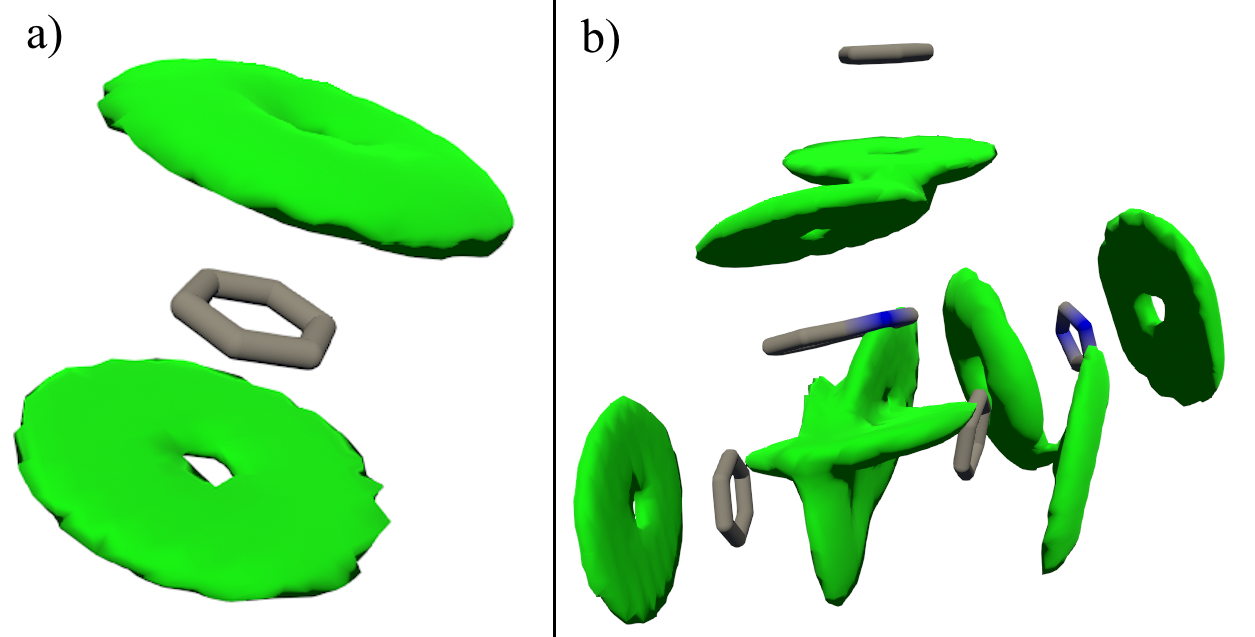
\includegraphics[width=0.7\textwidth]{figures/results/visualize_stacking.png}
        \caption{\label{fig:results/visualize_stacking} Isosurface representation of the stacking potential. a) tori of potential around a single aromatic ring, b) multiple tori around several aromatic rings. Only sphere trimming was performed, for clear visualization of the tori. Grid resolution: 50x50x50. Rendered in UnityMol.}
      \end{figure}

      The model is a sum of the potential distribution defined by each aromatic group, which means that in actual pockets more than one pair of tori can be present. These will naturally overlap with each other in regions where multiple aromatic groups are in close vicinity (figure \ref{fig:results/visualize_stacking}.b). Points were multiple tori intersect imply a higher propensity for a pharmacophore to form one or multiple stacking interactions, potentially from both sides of the aromatic plane. The trimming steps of the calculations will often cut out parts of the tori already occupied by the pocket atoms, so at the end the potential fields end up being mostly amorphous (e.g. figure \ref{fig:benchmark/1iqj}).

  \subsection{Hydrogen Bonds Potential}
    In the case of the hydrogen bonds potential, the function bases its univariate normal distributions only on distance. This simpler spatial constraint means that the potential value peaks at a given distance from the relevant atoms, which is the same in all directions. Intuitively, this generates a hollow shell around the atom, as can be seen in figure \ref{fig:results/visualize_hbonds}.a. Placing an acceptor or donor pharmacophore (whichever complements the target atom) in this shell means that a hydrogen bond interaction is plausible.

    \begin{figure}[H]
      \centering
      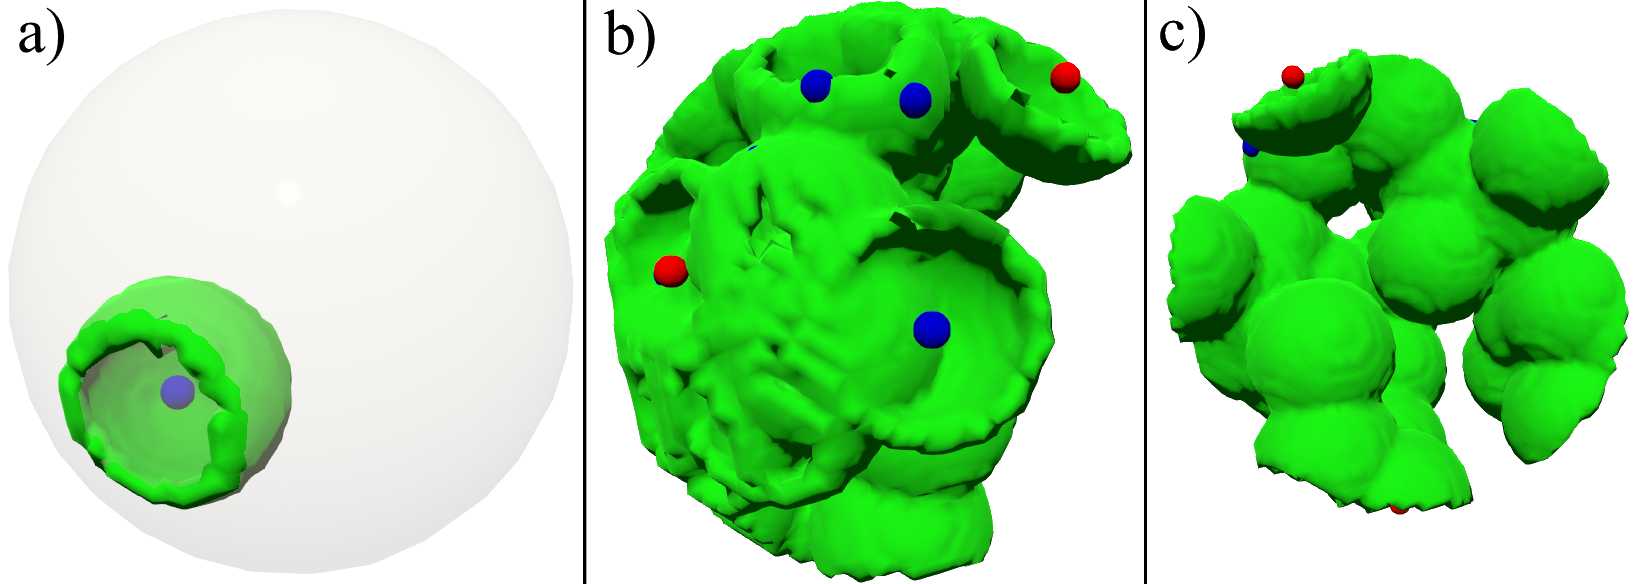
\includegraphics[width=1\textwidth]{figures/results/visualize_hbonds.png}
      \caption{\label{fig:results/visualize_hbonds} Isosurface representation of the hydrogen bonds acceptor potential. a) shell of potential around a single acceptor heteroatom, b) multiple shells around several plausible acceptors, c) different visualization angle for (b). Only sphere trimming was performed, for clear visualization of the shells. Grid resolution: 50x50x50. Rendered in UnityMol.}
    \end{figure}

    Similarly to the stacking potential, several shells will most likely overlap with each other when studying actual pockets (figures \ref{fig:results/visualize_hbonds}.b and \ref{fig:results/visualize_hbonds}.c). Placing a pharmacophore in these overlapping regions should further increase the propensity of a hydrogen bond interaction, as it implies there are more acceptor/donor candidates nearby.

    After trimming is performed, the surfaces defined by the hydrogen bond potential are further simplified and adopt an amorphous shape (e.g. figure \ref{fig:benchmark/1ofz}). Finally, due to the similarity of the potential functions, the hydrophobicity potential also yields similar spherical patterns, with the difference that these can have either positive or negative values (e.g. figure \ref{fig:benchmark/3dd0}).

  \subsection{Electrostatic Potential}
    As the electrostatic potential is based in a physical energy function, its output values are less linear than those of a statistical energy function and can vary between different orders of magnitude. Very high values occur in close proximity to atoms with partial charges, while the values quickly dissipate when moving towards the unoccupied volume of the pocket. In figure \ref{fig:results/logapbs_trimming} it can be observed that, even if most values are in an order of magnitude of around $1e1$ and $1e1.5$, some few points are present around $1e2.5$.

    \begin{figure}[H]
      \centering
      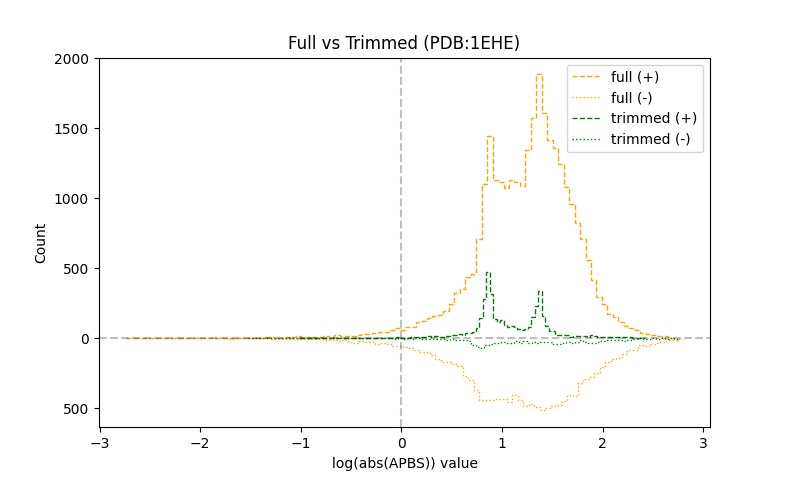
\includegraphics[width=0.7\textwidth]{figures/results/logapbs_trimming.png}
      \caption{\label{fig:results/logapbs_trimming} Distribution of negative and positive electric charges before and after the trimming steps.}
    \end{figure}

    This affects the cloud representation, as the colors and transparency depend on the normalized values of the potential: after normalization, only the few extreme values (around $1e2.5$) are displayed, while the majority of values inside the pocket (below $1e.5$) are drawn with a very low opacity. This is particularly evident when occupancy trimming is turned off, because a higher amount of extreme values near atoms remain unpruned (figure \ref{fig:results/logapbs_trimming}), and results in a highly focalized representation that is not very informative. This visual artifact is dubbed \textit{christmas tree effect} and is to be avoided (figure \ref{fig:results/apbs_christmas}.a).

    \begin{figure}[H]
      \centering
      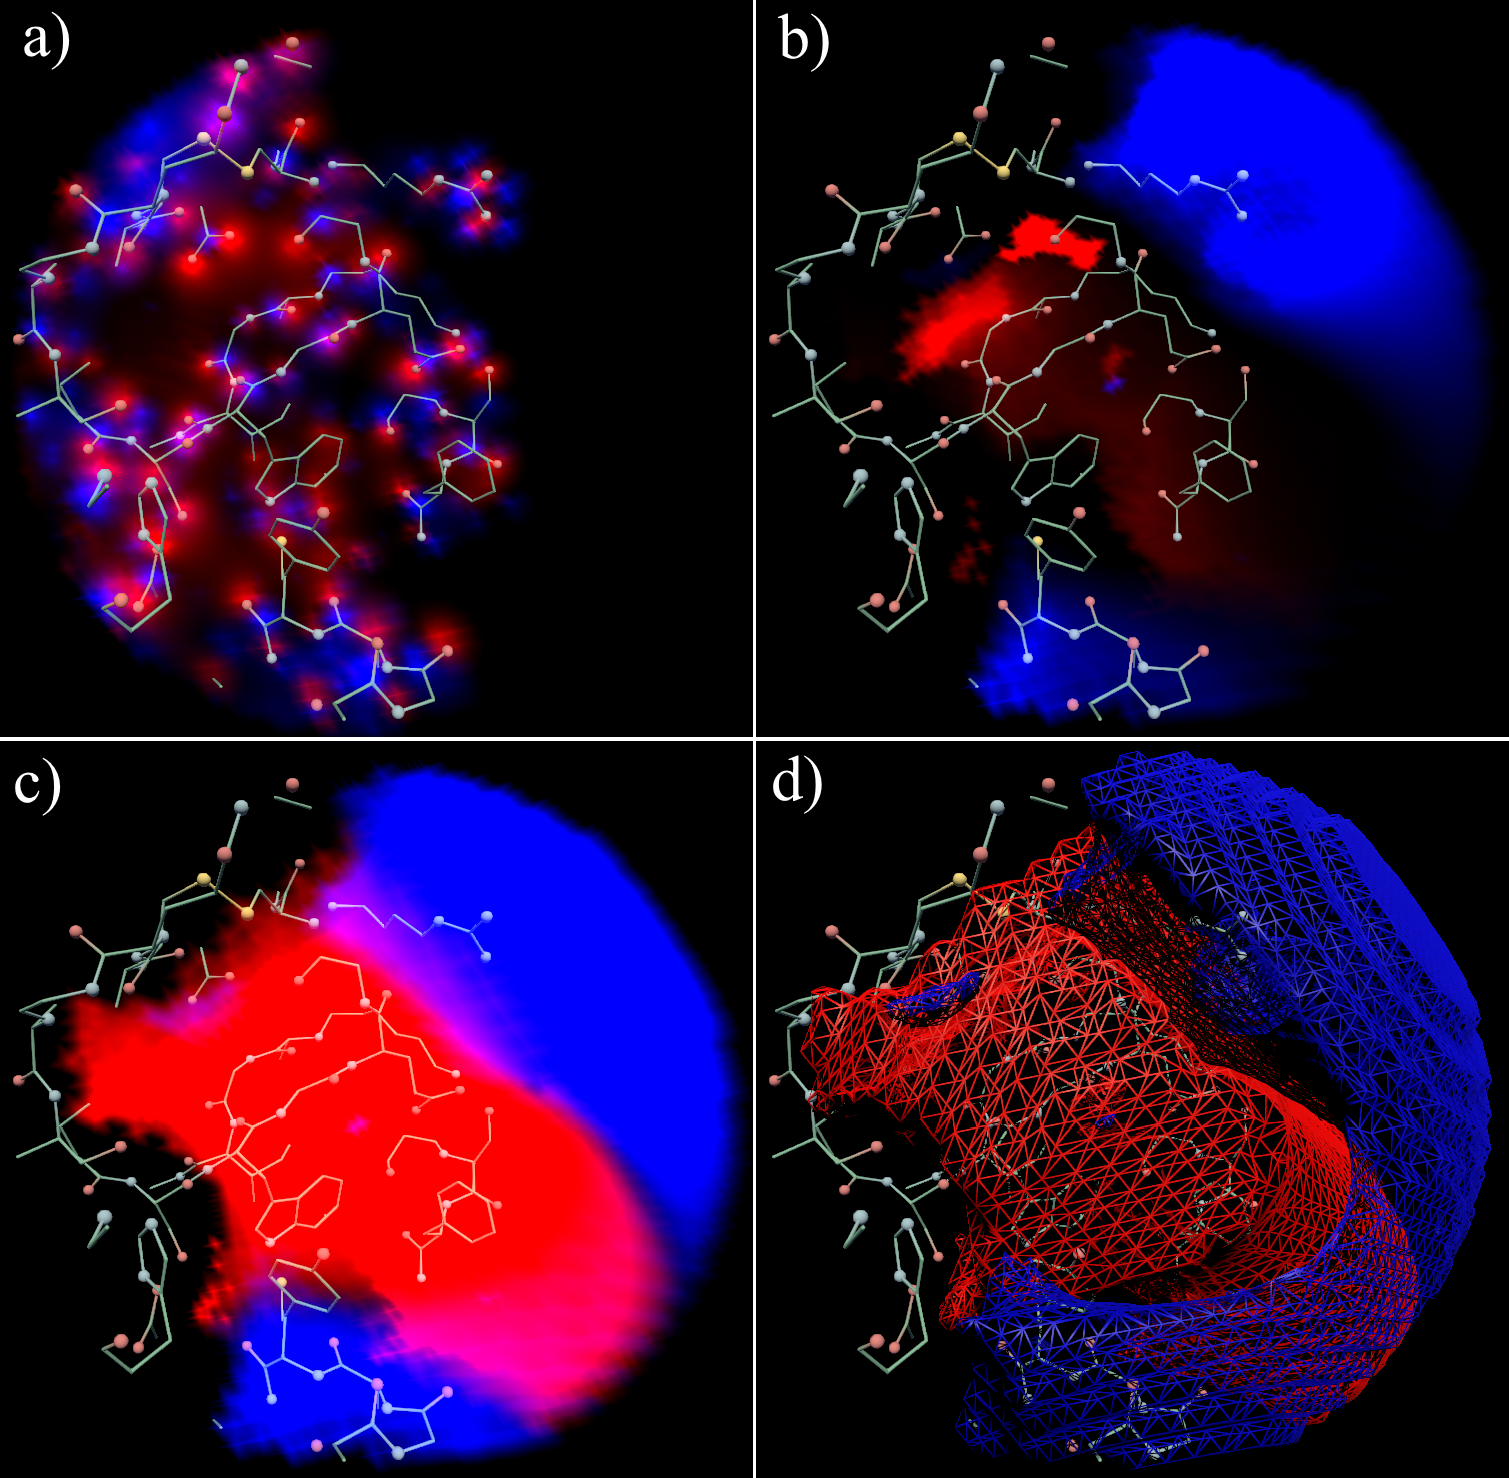
\includegraphics[width=0.7\textwidth]{figures/results/apbs_christmas.png}
      \caption{\label{fig:results/apbs_christmas} Visualization of the electrostatic potential under different conditions. a) cloud representation without trimming, b) cloud representation with trimming, c) cloud representation with trimming, log transformation applied, d) isosurfaces representation with trimming. PDB:1IQJ. Grid resolution: 52x49x46. Rendered in UnityMol.}
    \end{figure}

    Even if enabling occupancy trimming removes the majority of high values (figure \ref{fig:results/logapbs_trimming}), the presence of only a single value around $1e2.5$ is enough to influence on the normalization of colors and negatively affect the cloud representation in the same way (figure \ref{fig:results/apbs_christmas}.b). This problem is solved by either displaying the logarithmic transformation of the APBS values (figure \ref{fig:results/apbs_christmas}.c) or by using isosurfaces for either the original or log-transformed APBS values (figure \ref{fig:results/apbs_christmas}.d).


%%%%%%%%%%%%%%%%%%%%%%%%%%%%%%%%%%%%%%%%%%%%%%%%%%%%%%%%%%%%%%%%%%%%%%%%%%%%%%%%
\section{Development of Visualization Methods}
  \subsection{Graphical User Interface}
    The UnityMol GUI components were implemented for the PS pipeline, which allowed for easy manipulation of the pocket sphere size in real time, and provided both cartoon (figures \ref{fig:results/gui_sphere}.a and \ref{fig:results/gui_sphere}.b) and surface (figures \ref{fig:results/gui_sphere}.c and \ref{fig:results/gui_sphere}.d) representations of the system. It is important to note that the \textit{Extra size} slider of GUI becomes less reactive when setting the size of the pocket sphere to a large value, due to the atom selection calculations slowing down UnityMol. This slow-down is particularly noticeable when using the surface representation, as heavy calculations must be done when calculating each new variant of the surfaces. An example of usage of the GUI is provided in the appendix website at \url{https://diegobarmor.github.io/thesis-qcb/}

    \begin{figure}[H]
      \centering
      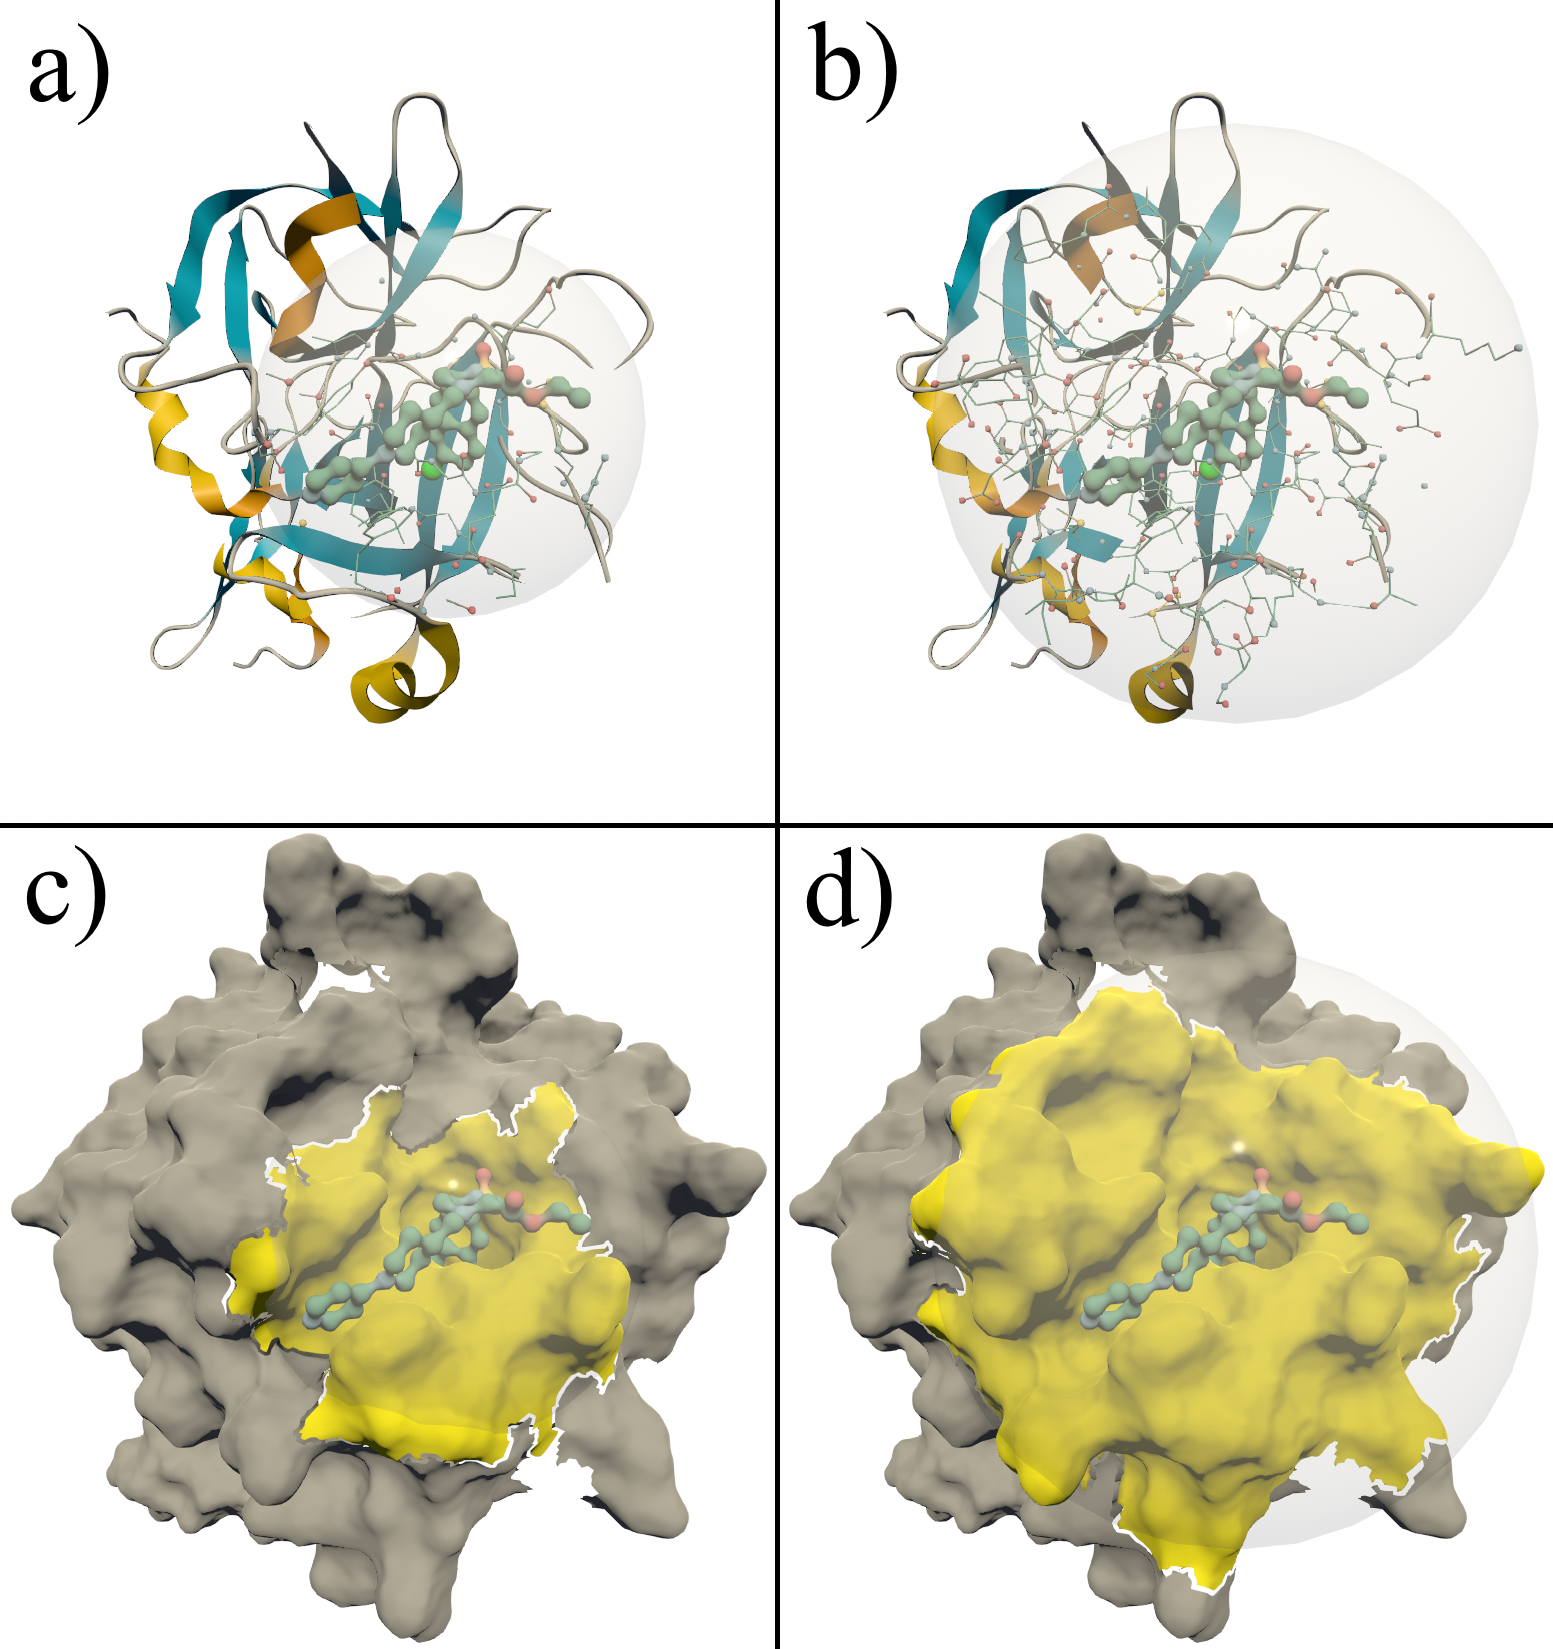
\includegraphics[width=0.6\textwidth]{figures/results/gui_sphere.png}
      \caption{\label{fig:results/gui_sphere} Interactive visualization of the pocket sphere (PS) in UnityMol. a and b) protein represented as cartoon, atoms inside the PS are highlighted as licorice, c and d) protein represented as surface, atoms inside the PS are highlighted in yellow. PS radius is increased by 10 in (b) and (d). PDB:1IQJ.}
    \end{figure}

  \subsection{Potentials Calculation}
    For any potentials calculation, performing the sphere and occupancy trimming is fundamental, as otherwise the visualization gets saturated with irrelevant datapoints (figure \ref{fig:results/trimming_0}). The RNDS trimming can be considered as an optional step for further polishing the visualization, at the expense of additional calculation time. An example of RNDS removing datapoints from a volume outside the pocket is presented in figure \ref{fig:results/trimming_1}. Further polishing can be performed by adding a threshold for the search distance, although this has to be done with care, to avoid removing relevant datapoints.

    \begin{figure}[H]
      \centering
      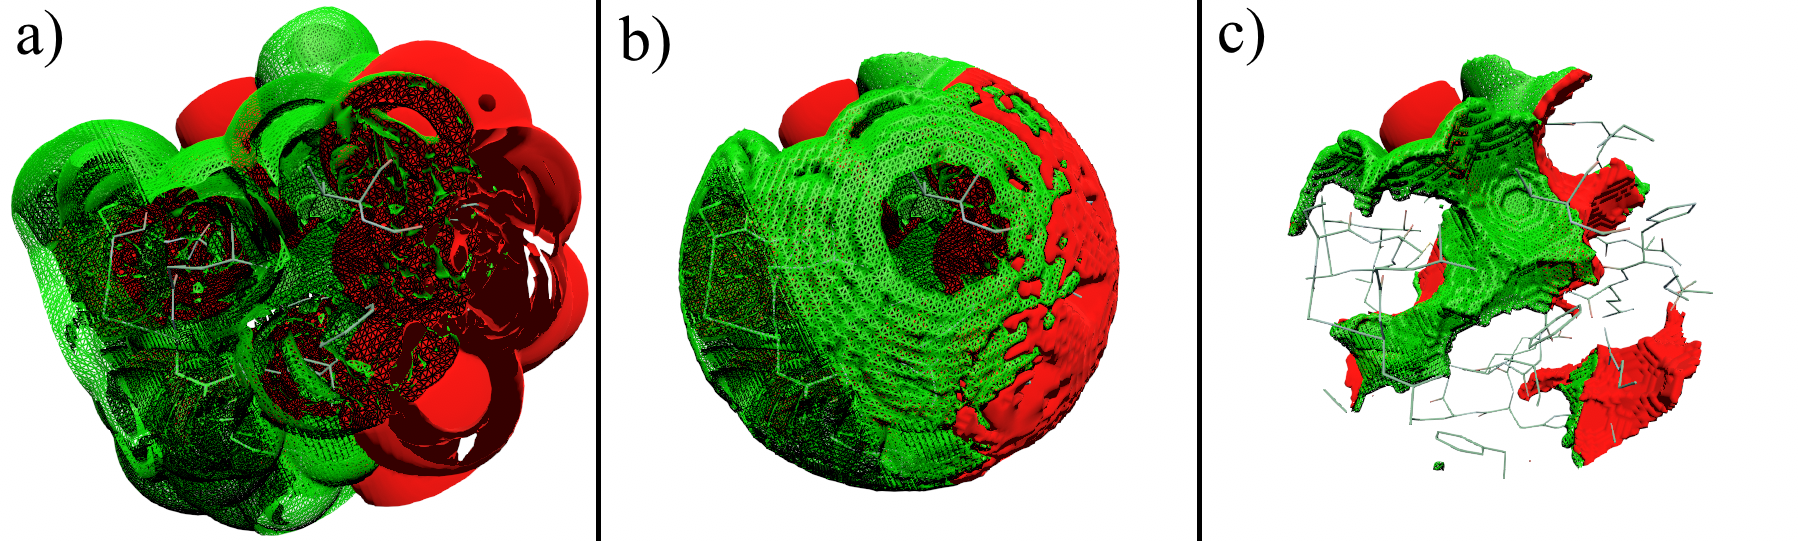
\includegraphics[width=1\textwidth]{figures/results/trimming_0.png}
      \caption{\label{fig:results/trimming_0} Trimming steps for the hydrophobicity potential (1/2). a) no trimming, b) sphere trimming, c) sphere and occupancy trimming. PDB:1EHE.}
    \end{figure}

    \begin{figure}[H]
      \centering
      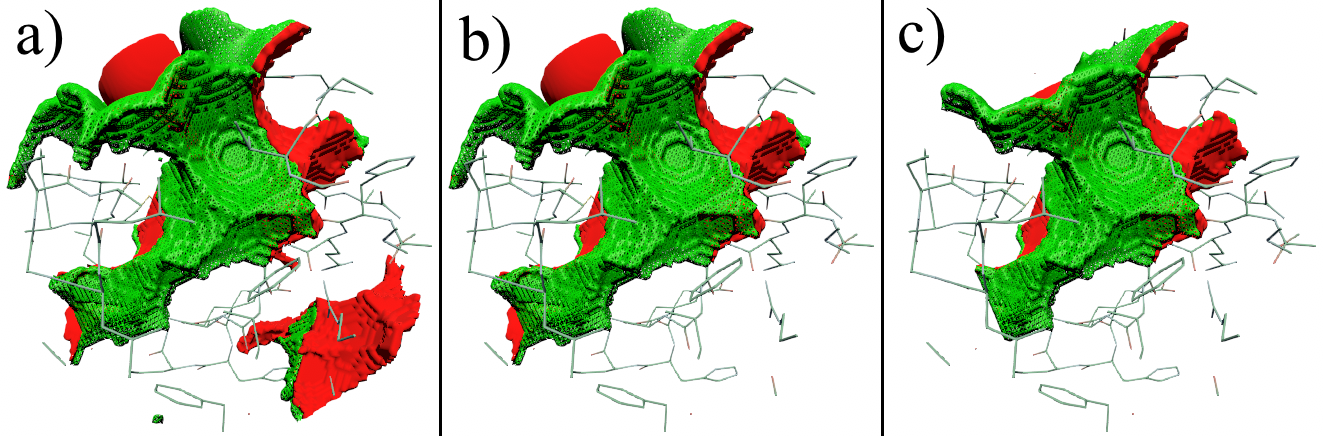
\includegraphics[width=1\textwidth]{figures/results/trimming_1.png}
      \caption{\label{fig:results/trimming_1} Trimming steps for the hydrophobicity potential (2/2). a) sphere and occupancy trimming, b) sphere, occupancy and RNDS trimming (no search distance threshold) c) sphere, occupancy and RNDS trimming (search distance threshold set to 35). PDB:1EHE.}
    \end{figure}

    Another important setting for the potentials calculation is the amount of points employed for calculating the grid, i.e. its resolution. A resolution of $50 \times 50 \times 50$ implies dealing with matrices of $125000$ datapoints, which are calculated relatively quickly (some seconds), but whose rendering consist of less intuitive shapes (figures \ref{fig:results/resolution}.a and \ref{fig:results/resolution}.c). A resolution of $100 \times 100 \times 100$ implies dealing with $1000000$ points, which increases the calculation time to the order of decaseconds, but which are displayed into better defined shapes and contours (figures \ref{fig:results/resolution}.b and \ref{fig:results/resolution}.d). It is also notable that the time for loading the matrix files and rendering the representations increases with the resolution, although not as extremely.

    \begin{figure}[H]
      \centering
      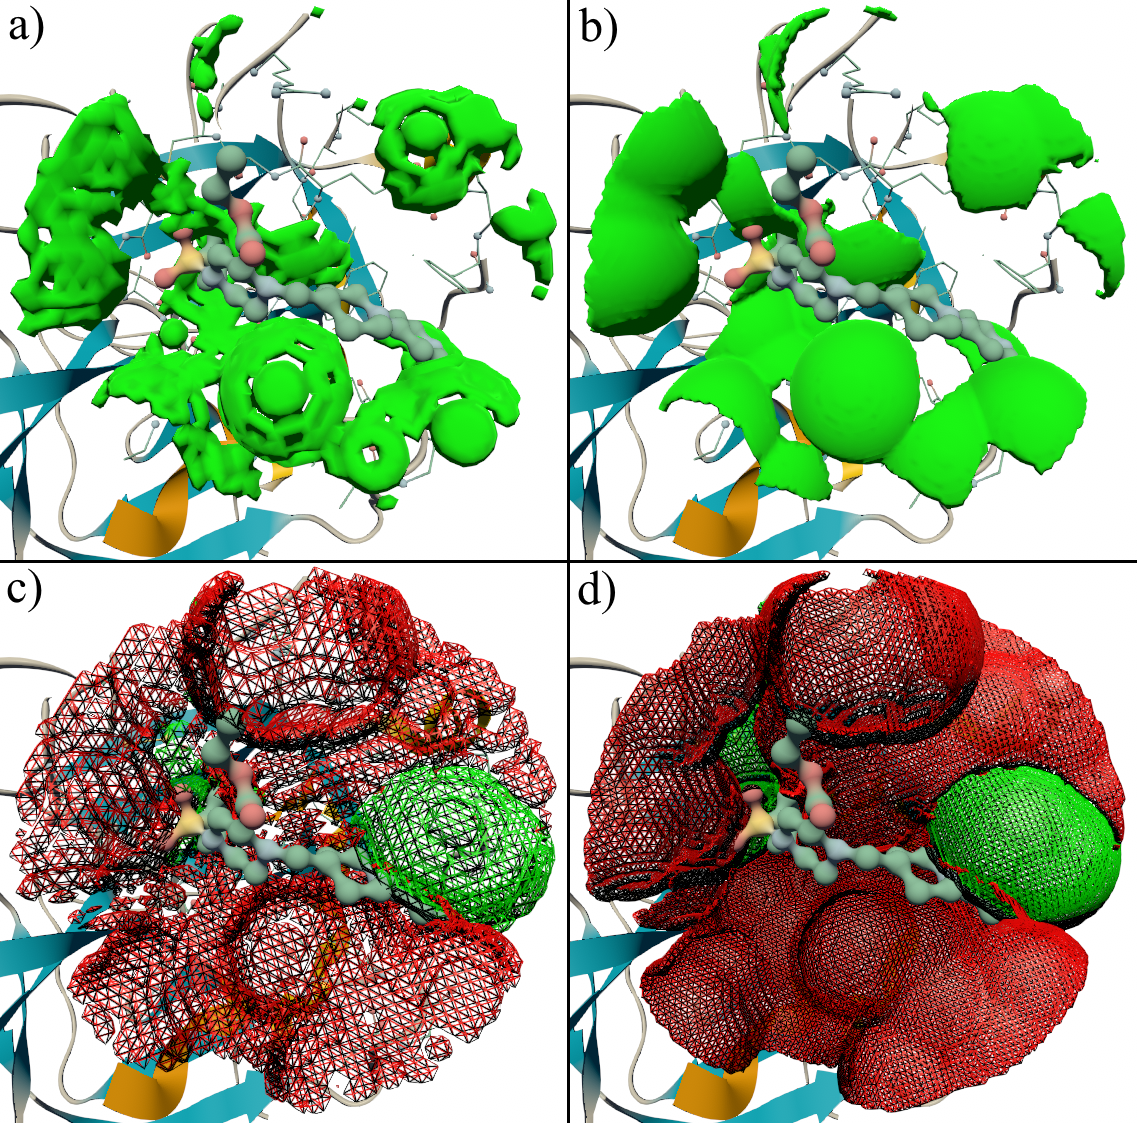
\includegraphics[width=0.6\textwidth]{figures/results/resolution.png}
      \caption{\label{fig:results/resolution} Effect of the resolution of the potential grids over the quality of the visualization. a) hydrogen bonds acceptor potential at resolution $50 \times 50 \times 50$, b) hydrogen bonds acceptor potential at resolution $100 \times 100 \times 100$, c) hydrophobic potential at resolution $50 \times 50 \times 50$, d) hydrophobic potential at resolution $100 \times 100 \times 100$. PDB:1IQJ.}
    \end{figure}

  \subsection{Potentials Visualization}
    Depending on the molecular system and the potentials to be visualized, different representation methods can be more convenient or ergonomic to use. For example, comparing the electrostatic potential of PDB:1EHE with its actual ligand position can be confusing when using only wireframe isosurfaces (figure \ref{fig:results/reprs_0}.c), as it ofuscates the ligand and the wireframe colors get mixed together. The cloud representation can be more useful for differentiating the electrostatic regions and the atoms below them, although it might still generate confusion (figure \ref{fig:results/reprs_0}.a). In this particular example, an appropriate intermediate option is mixing solid and translucid isosurfaces (figure \ref{fig:results/reprs_0}.b).

    \begin{figure}[H]
      \centering
      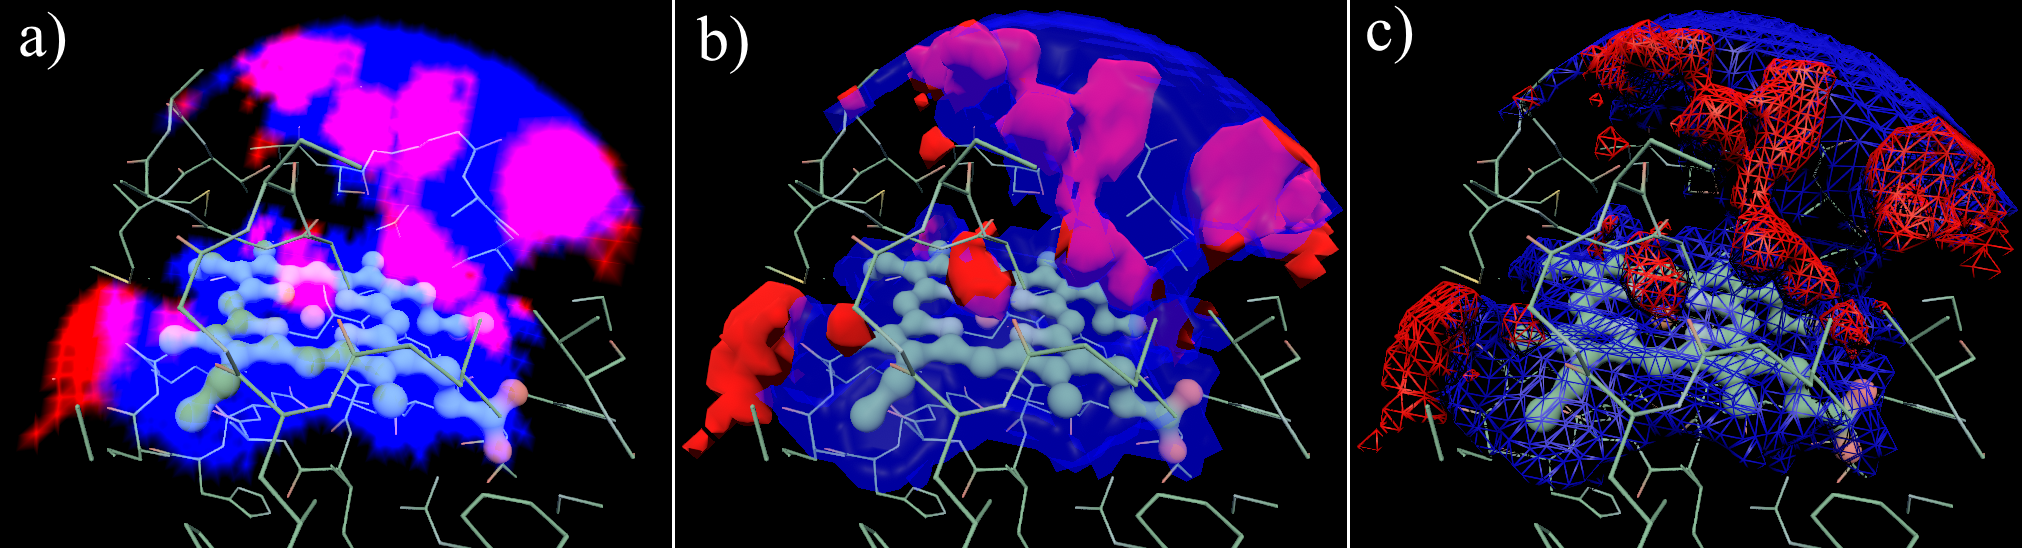
\includegraphics[width=0.8\textwidth]{figures/results/reprs_0.png}
      \caption{\label{fig:results/reprs_0} Different representations for visualizing the electrostatic potential. a) cloud representation, b) opaque and translucid isosurfaces, c) wireframe isosurfaces. PDB:1EHE.}
    \end{figure}

    In the case of the stacking potential, comparing the ligand position is even harder when using solid or wireframe isosurfaces, as it is difficult to distinguish the aromatic rings overlapping with the potential (figures \ref{fig:results/reprs_1}.c and \ref{fig:results/reprs_1}.d), while translucid and cloud are more appropriate for this purpose (figures \ref{fig:results/reprs_1}.a and \ref{fig:results/reprs_1}.b). Note however that, if the actual potential shape of is of interest and the ligand is disregarded, the solid and wireframe isosurfaces are a better choice. Also note that the cloud representation in figure \ref{fig:results/reprs_1}.a gives less relevance to low value subregions (which can be considered noise), while the translucid isosurface from figure \ref{fig:results/reprs_1}.b gives the same homogeneous color to all points, regardless of their potential value.

    \begin{figure}[H]
      \centering
      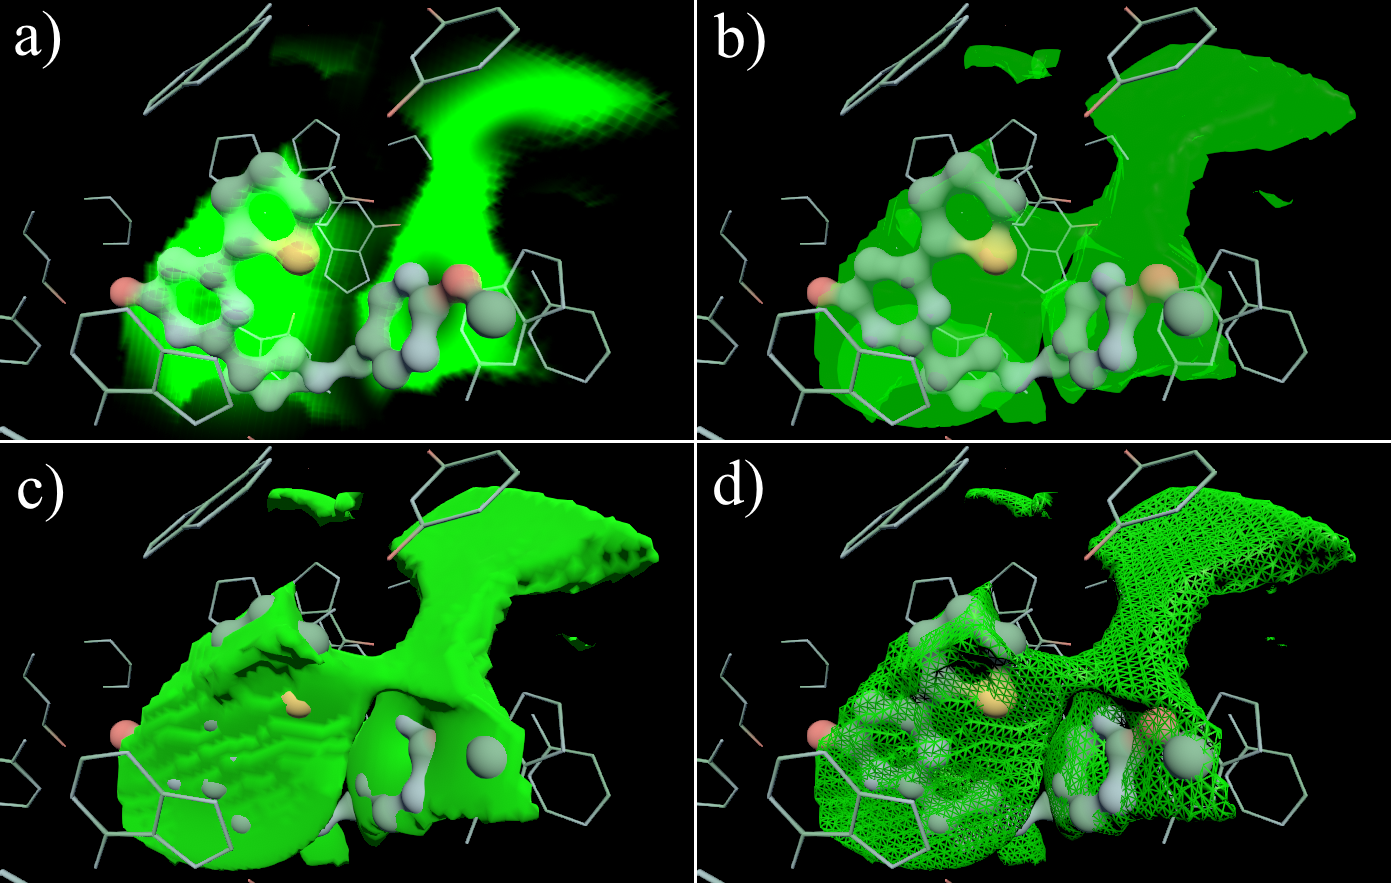
\includegraphics[width=0.6\textwidth]{figures/results/reprs_1.png}
      \caption{\label{fig:results/reprs_1} Different representations for visualizing the stacking potential. a) cloud representation, b) translucid isosurface, c) opaque isosurface, d) wireframe isosurface. PDB:5KX9.}
    \end{figure}

    Even if the hydrogen bond potential have some resemblances with the stacking potential in its calculation, the practicality of its representation differs. The cloud and translucid representations are usually vague and not very intuitive (figures \ref{fig:results/reprs_2}.a and \ref{fig:results/reprs_2}.b), while the solid and wireframe representations are most likely to be preferred (figures \ref{fig:results/reprs_2}.c and \ref{fig:results/reprs_2}.d). This is due to the fact that these potentials are closer to the actual surface of the target (while the stacking extends towards the pocket center), so the ligand or pharmacophore is less obstructed during the visualization. The spherical shapes from this potential are also very evident in the solid isosurfaces.

    \begin{figure}[H]
      \centering
      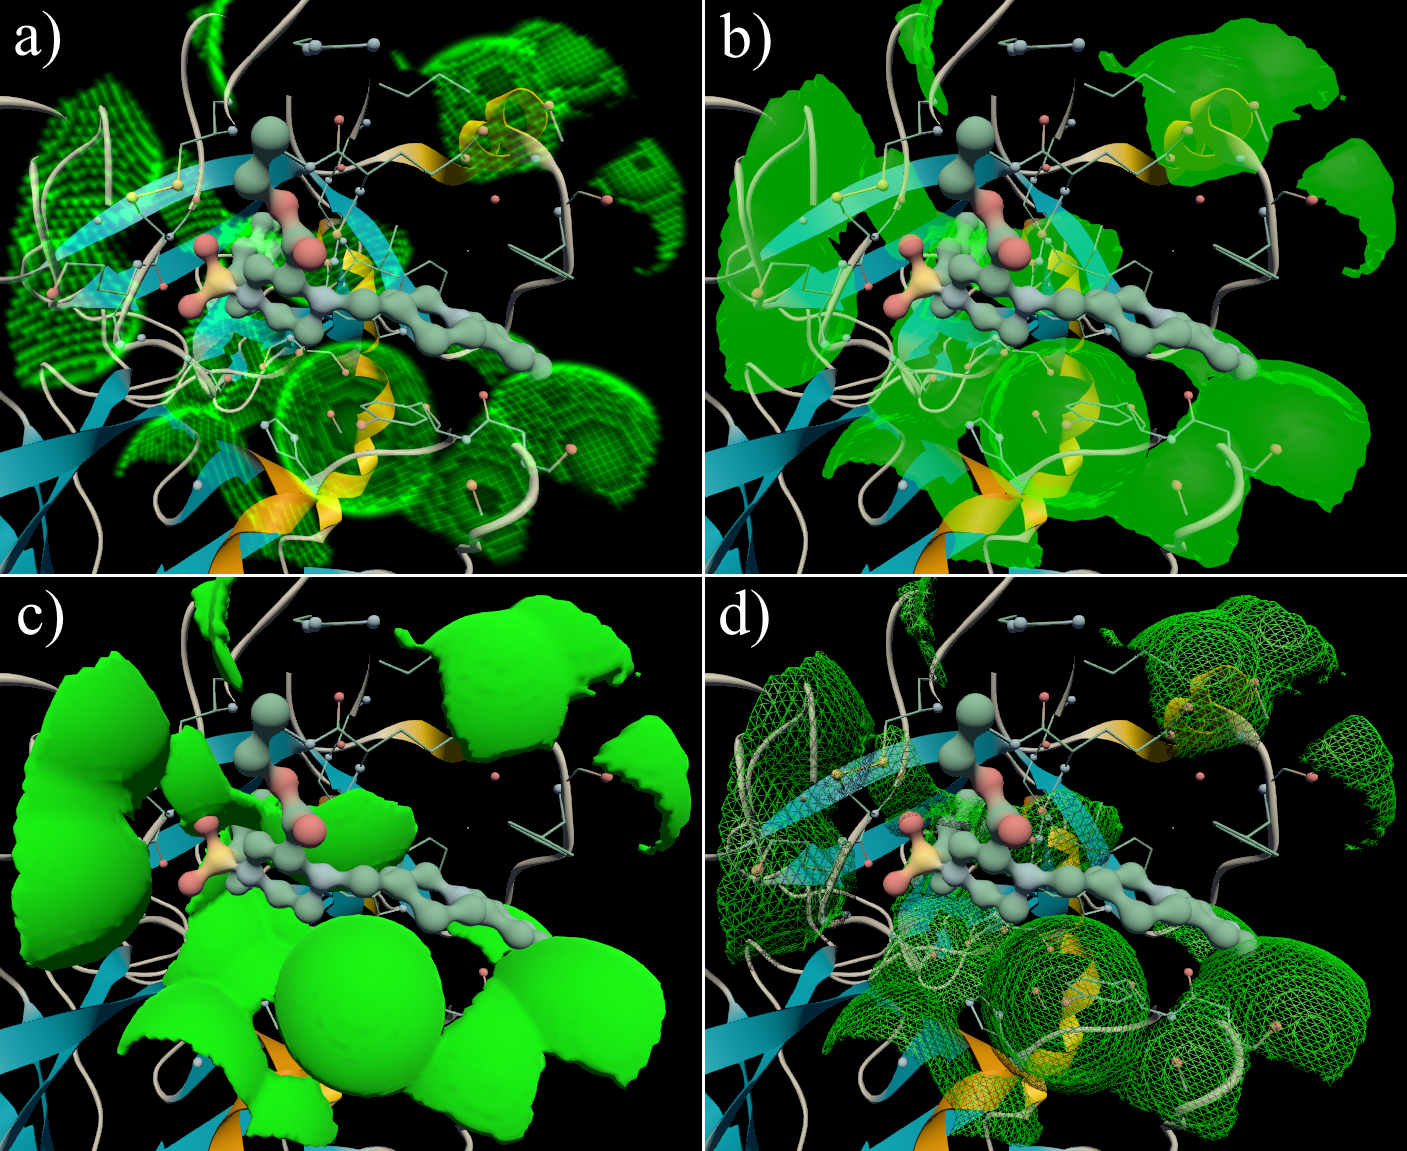
\includegraphics[width=0.8\textwidth]{figures/results/reprs_2.png}
      \caption{\label{fig:results/reprs_2} Different representations for visualizing the hydrogen bonds acceptor potential. a) cloud representation, b) translucid isosurface, c) opaque isosurface, d) wireframe isosurface. PDB:1IQJ.}
    \end{figure}

    A final observation regarding the isosurface representations is that the user must deal with the \textit{isovalue} parameter, which can be unintuitive and generate confusion about the actual meaning of the rendered shapes. On the other hand, being able to change this parameter allows to better adjust each particular case, even if the underlying technical concept of an isovalue is not clear to the user. The cloud representation lacks this issue.


%%%%%%%%%%%%%%%%%%%%%%%%%%%%%%%%%%%%%%%%%%%%%%%%%%%%%%%%%%%%%%%%%%%%%%%%%%%%%%%%
\section{Benchmarking}
  In this section, a highlight of the most interesting benchmark observations is given. For each system, a 3D representation of the complete macromolecule (with its pocket highlighted in orange) and a 2D schema of the ligand are also provided. A complete list of all potential visualization for all the benchmarks is provided in Appendix II. This complete list is also available at high definition in the appendix website at \url{https://diegobarmor.github.io/thesis-qcb/}.

  In the case of RNA systems, all of the 10 benchmarks present electronegative pockets (sometimes with few negligible positive points), so only observations regarding stacking and hydrogen bond potentials will be discussed. For each system, the ligand atoms found to be relevant by PLIP (table \ref{tab:appx2/plip}) are emphasized, noting whether or not they overlap with regions of hydrogen bond potentials. In the case of stacking, the role of relevant RNA residues (according to PLIP) are also compared to what can be inferred from their respective stacking potential visualization.

  \pagebreak
  \subsection{Protein Systems}
    \subsubsection{1BG0: Arginine kinase bound to ADP}
      \begin{figure}[H] \centering
        \begin{subfigure}[c]{0.3\textwidth} \centering
          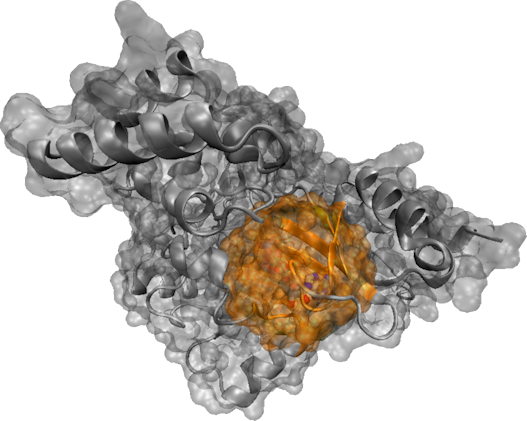
\includegraphics[width=1\textwidth]{figures/results/ps_prot/1bg0.png}
        \end{subfigure}
        \begin{subfigure}[c]{0.3\textwidth} \centering
          \psfig{file=figures/results/ligands/ADP.eps, width=1\textwidth}
        \end{subfigure}
      \end{figure}

      Electrostatic interactions are known to play an important role in the binding site of this protein. The negatively charged phosphate groups of the ligand interact with positively charged arginines, while aminoacids such as glutamate and aspartate form an electronegative cluster that interacts with a magnesium cation (necessary to stabilize the complex) \cite{benchmark_negative_2000}.

      It can be observed in figure \ref{fig:benchmark/1bg0} that the phosphate group of the ligand occupies an electropositive region of the pocket, while the magnesium cation is accurately placed in an electronegative region provided by the highlighted glutamates. This is congruent with the expected electrostatic interactions. Furthermore, figure \ref{fig:appx_benchmark/1bg0} shows how the aromatic group of the ligand aligns with one of the few regions of stacking potentials, while multiple oxygen and nitrogen atoms overlap with gridpoints for hydrogen bond potentials. Most of the pocket is hydrophilic, which is where the ligand, NO3 group and the ion are located.

      \begin{figure}[H]
        \centering
        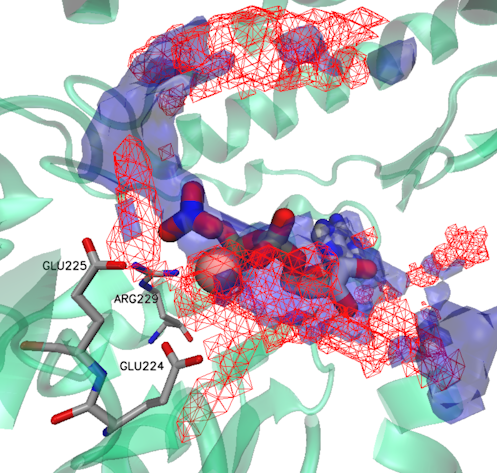
\includegraphics[width=0.5\textwidth]{figures/results/benchmark_prot/1bg0.png}
        \caption{\label{fig:benchmark/1bg0} Electrostatic potential of the pocket for the protein system PDB:1BG0.}
      \end{figure}
    \pagebreak

    \subsubsection{1EBY: HIV-1 protease in complex with the inhibitor BEA369}
      \begin{figure}[H] \centering
        \begin{subfigure}[c]{0.3\textwidth} \centering
          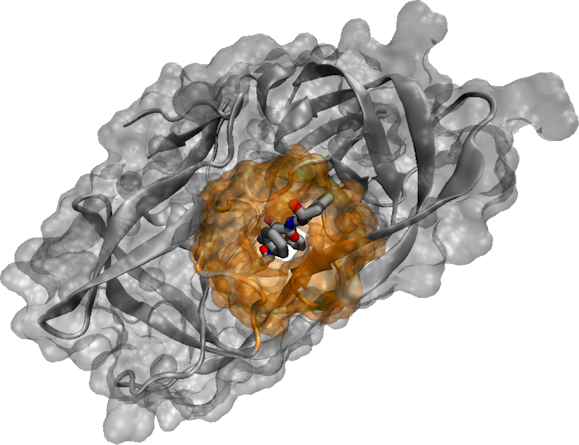
\includegraphics[width=1\textwidth]{figures/results/ps_prot/1eby.png}
        \end{subfigure}
        \begin{subfigure}[c]{0.3\textwidth} \centering
          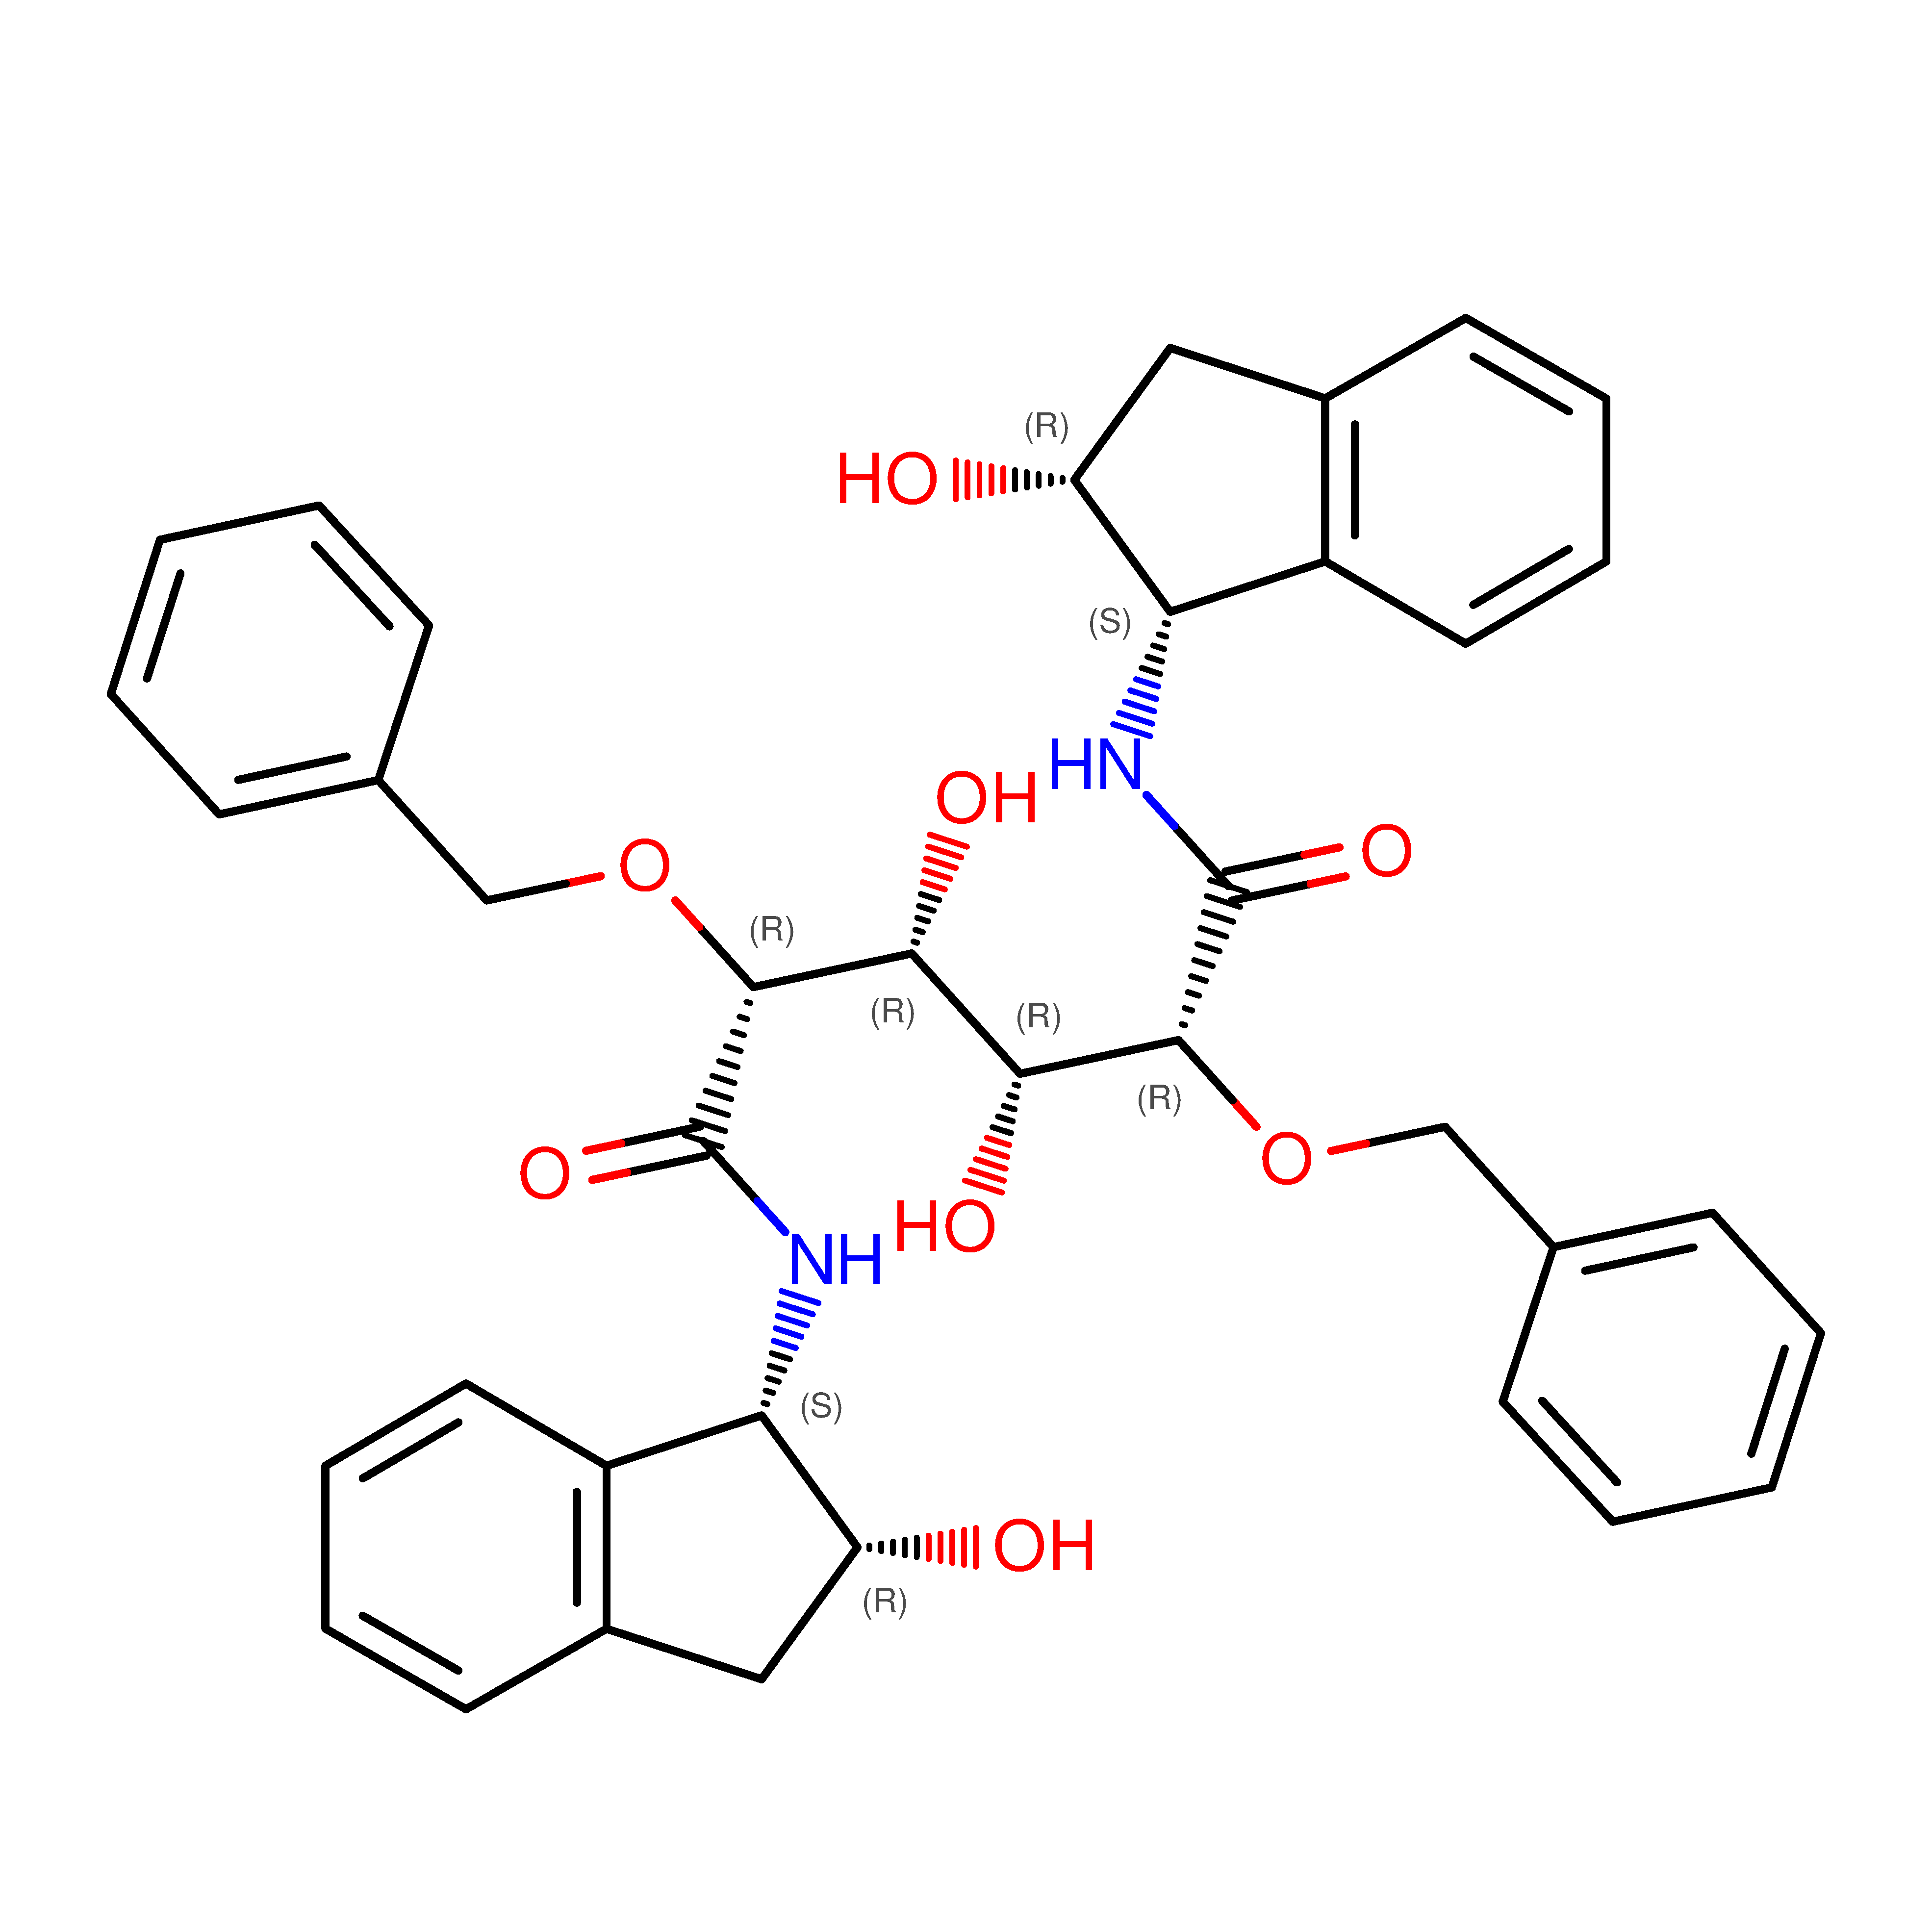
\psfig{file=figures/results/ligands/BEB.eps, width=1\textwidth}
        \end{subfigure}
      \end{figure}

      The strong binding affinity reported for this system is mostly due to the large amount of hydrogen bonds and hydrophobic interactions formed between the pocket and the ligand \cite{benchmark_strong_2021}. The hydrophobicity potential grid has the particularity that the hydrophobic and hydrophilic grid points are so intertwined, it is better to visualize them separately (figure \ref{fig:benchmark/1eby}). The hydrophobic region tends to overlap with the non-polar aromatic groups of the ligand, while the hydrophilic region overlaps more with the oxygen and nitrogen atoms. This makes sense in terms of hydrophobic interactions and coincides with what has been reported before \cite{benchmark_strong_2021}.

      The hydrogen bond potentials (figure \ref{fig:appx_benchmark/1eby}) also overlap with the atoms reported by \cite{benchmark_strong_2021}. As additional remarks, the protein lacks aromatic groups inside the pocket sphere, so there is no stacking potential in this case. The pocket is mostly electronegative with some positive points (figure \ref{fig:appx_benchmark/1eby}).

      \begin{figure}[H]
        \centering
        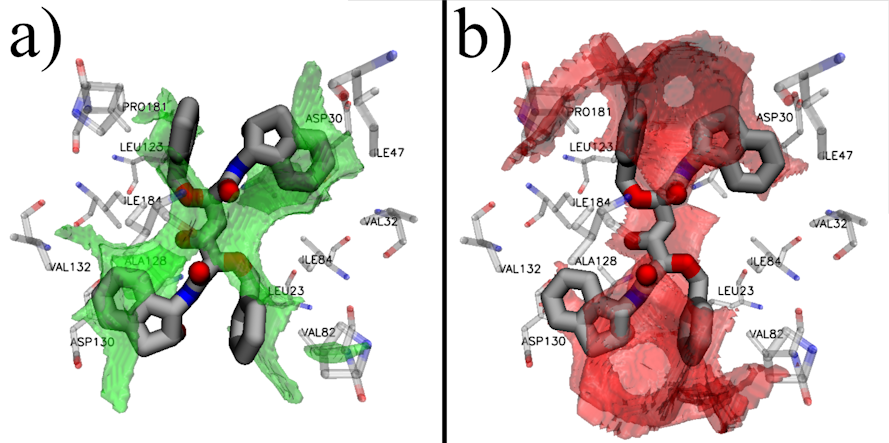
\includegraphics[width=0.7\textwidth]{figures/results/benchmark_prot/1eby.png}
        \caption{\label{fig:benchmark/1eby} Physical properties of the pocket for the protein system PDB:1EBY. Potentials displayed: a) hydrophobicity, b) hydrophilicity.}
      \end{figure}
    \pagebreak

    \subsubsection{1EHE: Monooxygenase cytochrome P450S bound to a heme group with iron}
      \begin{figure}[H] \centering
        \begin{subfigure}[c]{0.3\textwidth} \centering
          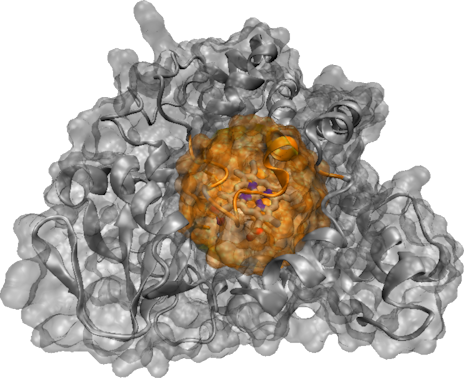
\includegraphics[width=1\textwidth]{figures/results/ps_prot/1ehe.png}
        \end{subfigure}
        \begin{subfigure}[c]{0.3\textwidth} \centering
          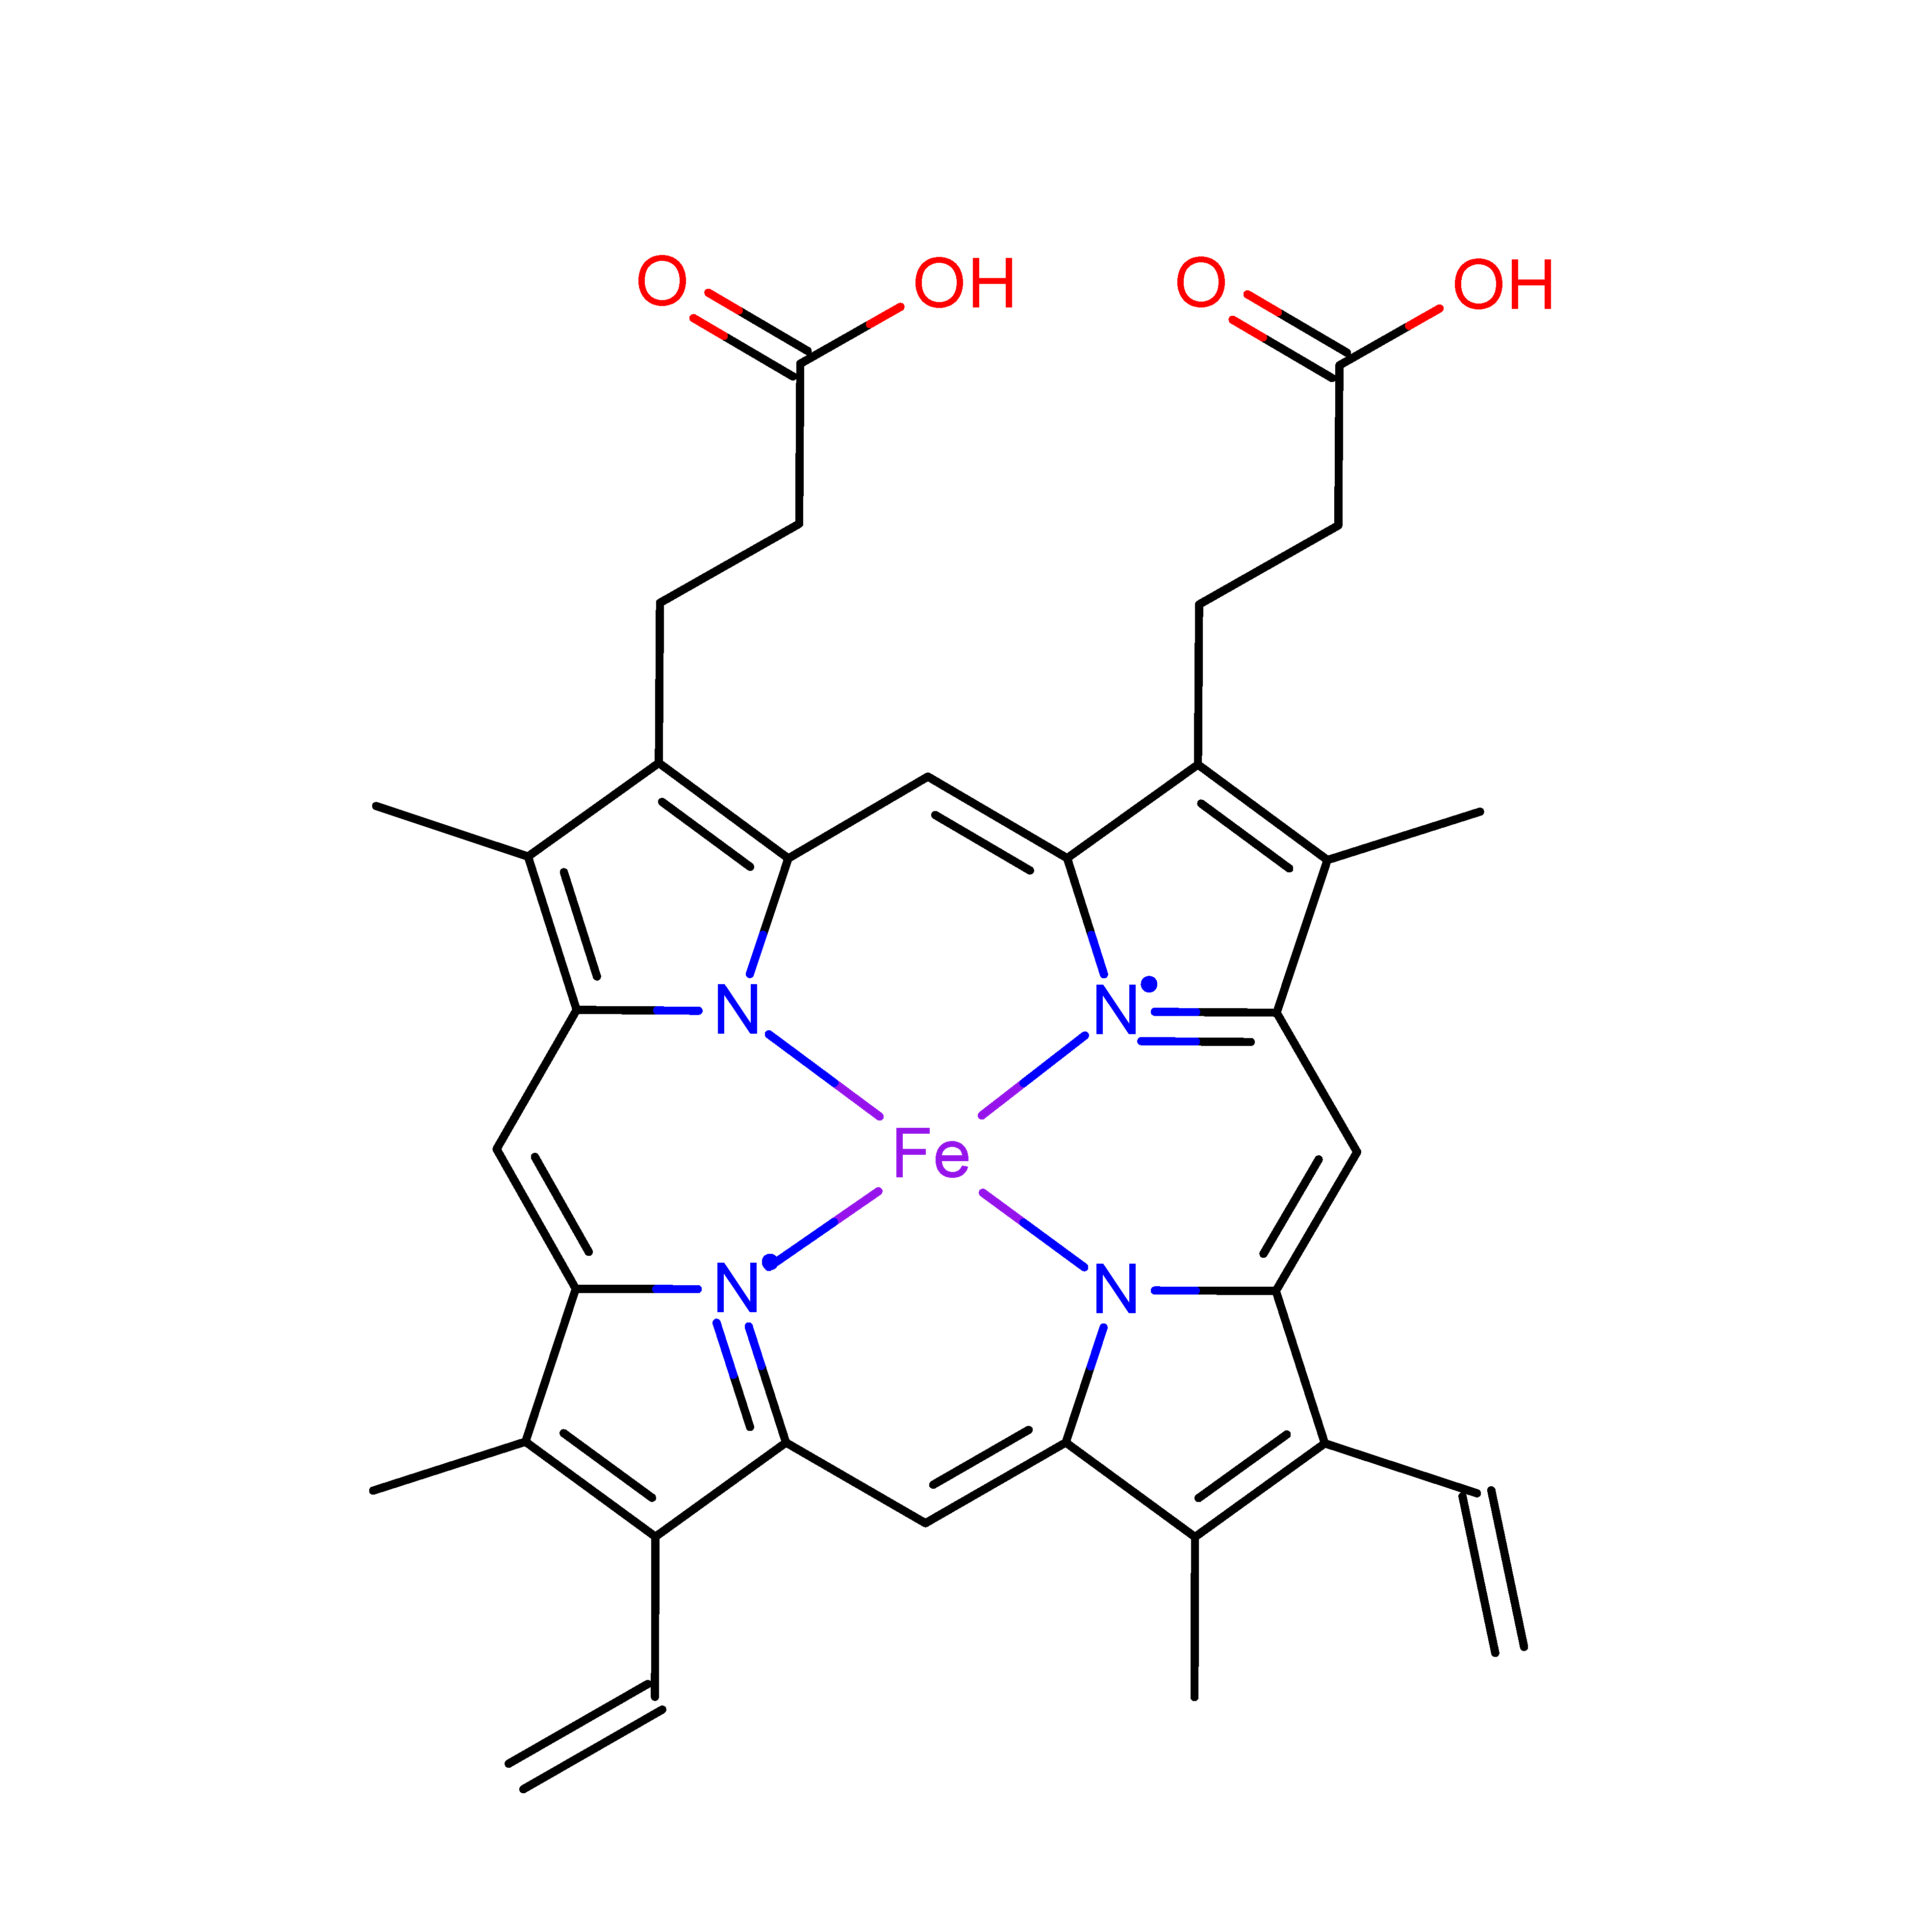
\psfig{file=figures/results/ligands/HEM.eps, width=1\textwidth}
        \end{subfigure}
      \end{figure}

      The binding pocket of this protein is characterized by a positively charged cluster of lysine and arginine residues, which plays an important role on how it interacts with the heme group ligand \cite{benchmark_positive_2001}. Indeed, the visualization of the electrostatic potential reveals positive charges in the region where the ligand should be placed. Furthermore, a negative charge can be observed overlapping with the cation in the middle of the heme group, which is to be expected (figure \ref{fig:benchmark/1ehe}).

      Additional observations include the stacking potential slightly overlapping with one of the aromatic groups, while the hydrogen bond potentials are displayed on top of the ligand's heteroatoms. The hydrophobic main body of the ligand overlaps with a large region of hydrophobic potential, while the outside oxygen atoms are placed inside hydrophilic sections (figure \ref{fig:appx_benchmark/1ehe}).

      \begin{figure}[H]
        \centering
        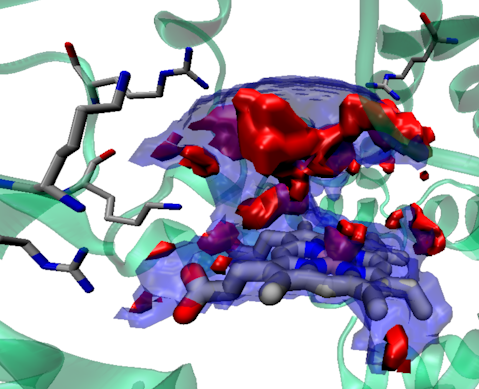
\includegraphics[width=0.5\textwidth]{figures/results/benchmark_prot/1ehe.png}
        \caption{\label{fig:benchmark/1ehe} Electrostatic potential of the pocket for the protein system PDB:1EHE.}
      \end{figure}
    \pagebreak

    \subsubsection{1H7L: Glycosyltransferase SpsA in complex with dTDP and magnesium}
      \begin{figure}[H] \centering
        \begin{subfigure}[c]{0.3\textwidth} \centering
          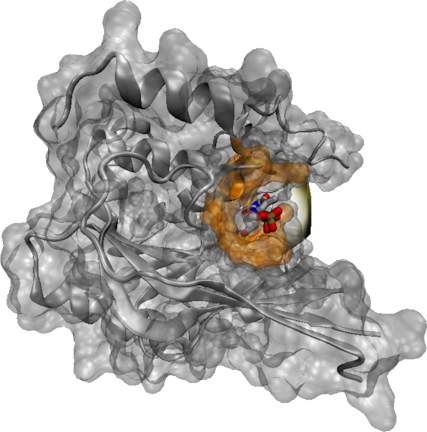
\includegraphics[width=1\textwidth]{figures/results/ps_prot/1h7l.png}
        \end{subfigure}
        \begin{subfigure}[c]{0.3\textwidth} \centering
          \psfig{file=figures/results/ligands/TYD.eps, width=1\textwidth}
        \end{subfigure}
      \end{figure}

      One of the main interactions required for the catalytic activity of this protein is the formation of a hydrogen bond between an aspartate and the hydroxylic group of the ligand \cite{benchmark_1h7l_2001}. Indeed, this interaction is hinted in figure \ref{fig:benchmark/1h7l}.

      The other potential grids describe the pocket as mostly electronegative and hydrophilic. A region of stacking potential overlaps with the aromatic thymidine group, while the rest of the hydrogen bond potentials do not seem to overlap much with the ligand's heteroatoms (figure \ref{fig:appx_benchmark/1h7l}).

      \begin{figure}[H]
        \centering
        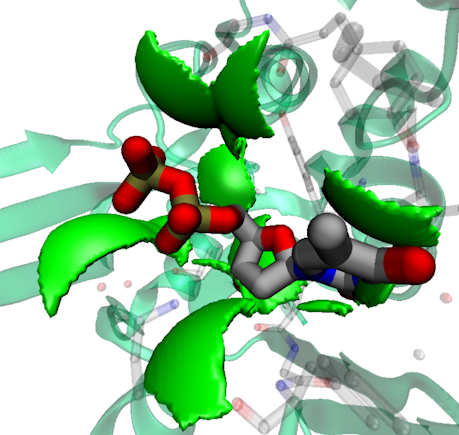
\includegraphics[width=0.5\textwidth]{figures/results/benchmark_prot/1h7l.png}
        \caption{\label{fig:benchmark/1h7l} Hydrogen bond acceptors potential of the pocket for the protein system PDB:1H7L.}
      \end{figure}
    \pagebreak

    \subsubsection{1IQJ: Human coagulation factor Xa in complex with M55124}
      \begin{figure}[H] \centering
        \begin{subfigure}[c]{0.3\textwidth} \centering
          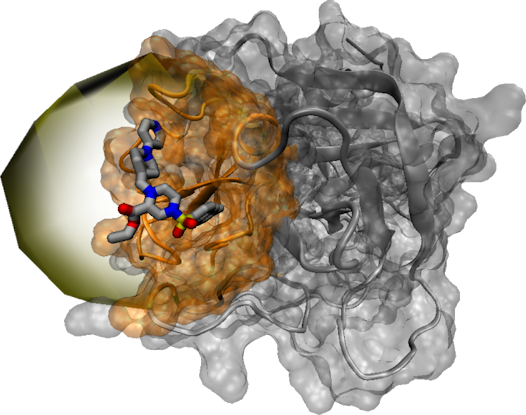
\includegraphics[width=1\textwidth]{figures/results/ps_prot/1iqj.png}
        \end{subfigure}
        \begin{subfigure}[c]{0.3\textwidth} \centering
          \psfig{file=figures/results/ligands/XMH.eps, width=1\textwidth}
        \end{subfigure}
      \end{figure}

      The ligand's aromatic pyridine group can be seen positioned in a significant stacking potential region (figure \ref{fig:benchmark/1iqj}). It can be easily inferred from the representation that this pyridine performs an aromatic interaction from both sides of the aromatic plane, hence the preference of this positioning.

      The electrostatics of the pocket form an interesting shape, with the ligand being present in an electronegative region surrounded by positive charges. Most of the pocket is hydrophilic, while the few hydrophobic sections neatly connect with the most hydrophobic parts of the ligand. Finally, the hydrogen bond potentials do not seem to interact much with the ligand's heteroatoms (figure \ref{fig:appx_benchmark/1iqj}).

      \begin{figure}[H]
        \centering
        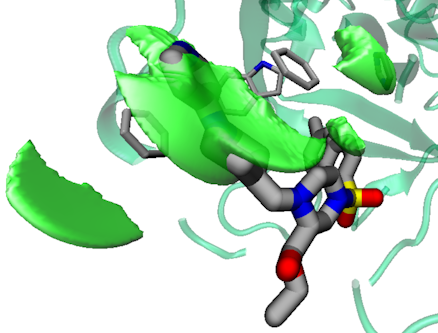
\includegraphics[width=0.5\textwidth]{figures/results/benchmark_prot/1iqj.png}
        \caption{\label{fig:benchmark/1iqj} Stacking potential of the pocket for the protein system PDB:1IQJ.}
      \end{figure}
    \pagebreak

    \subsubsection{1OFZ: Fungal lectin bound to beta-L-fucopyranose}
      \begin{figure}[H] \centering
        \begin{subfigure}[c]{0.3\textwidth} \centering
          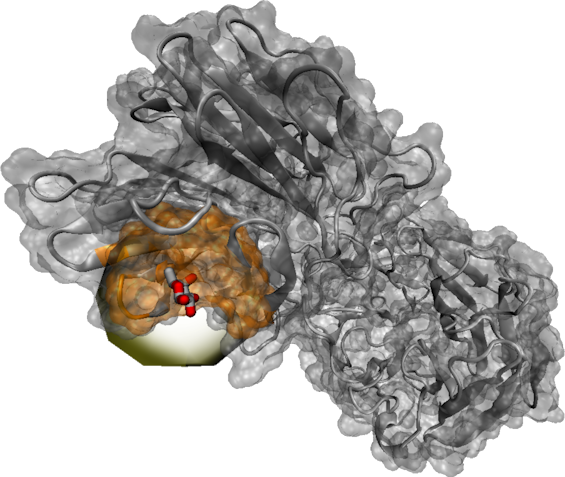
\includegraphics[width=1\textwidth]{figures/results/ps_prot/1ofz.png}
        \end{subfigure}
        \begin{subfigure}[c]{0.3\textwidth} \centering
          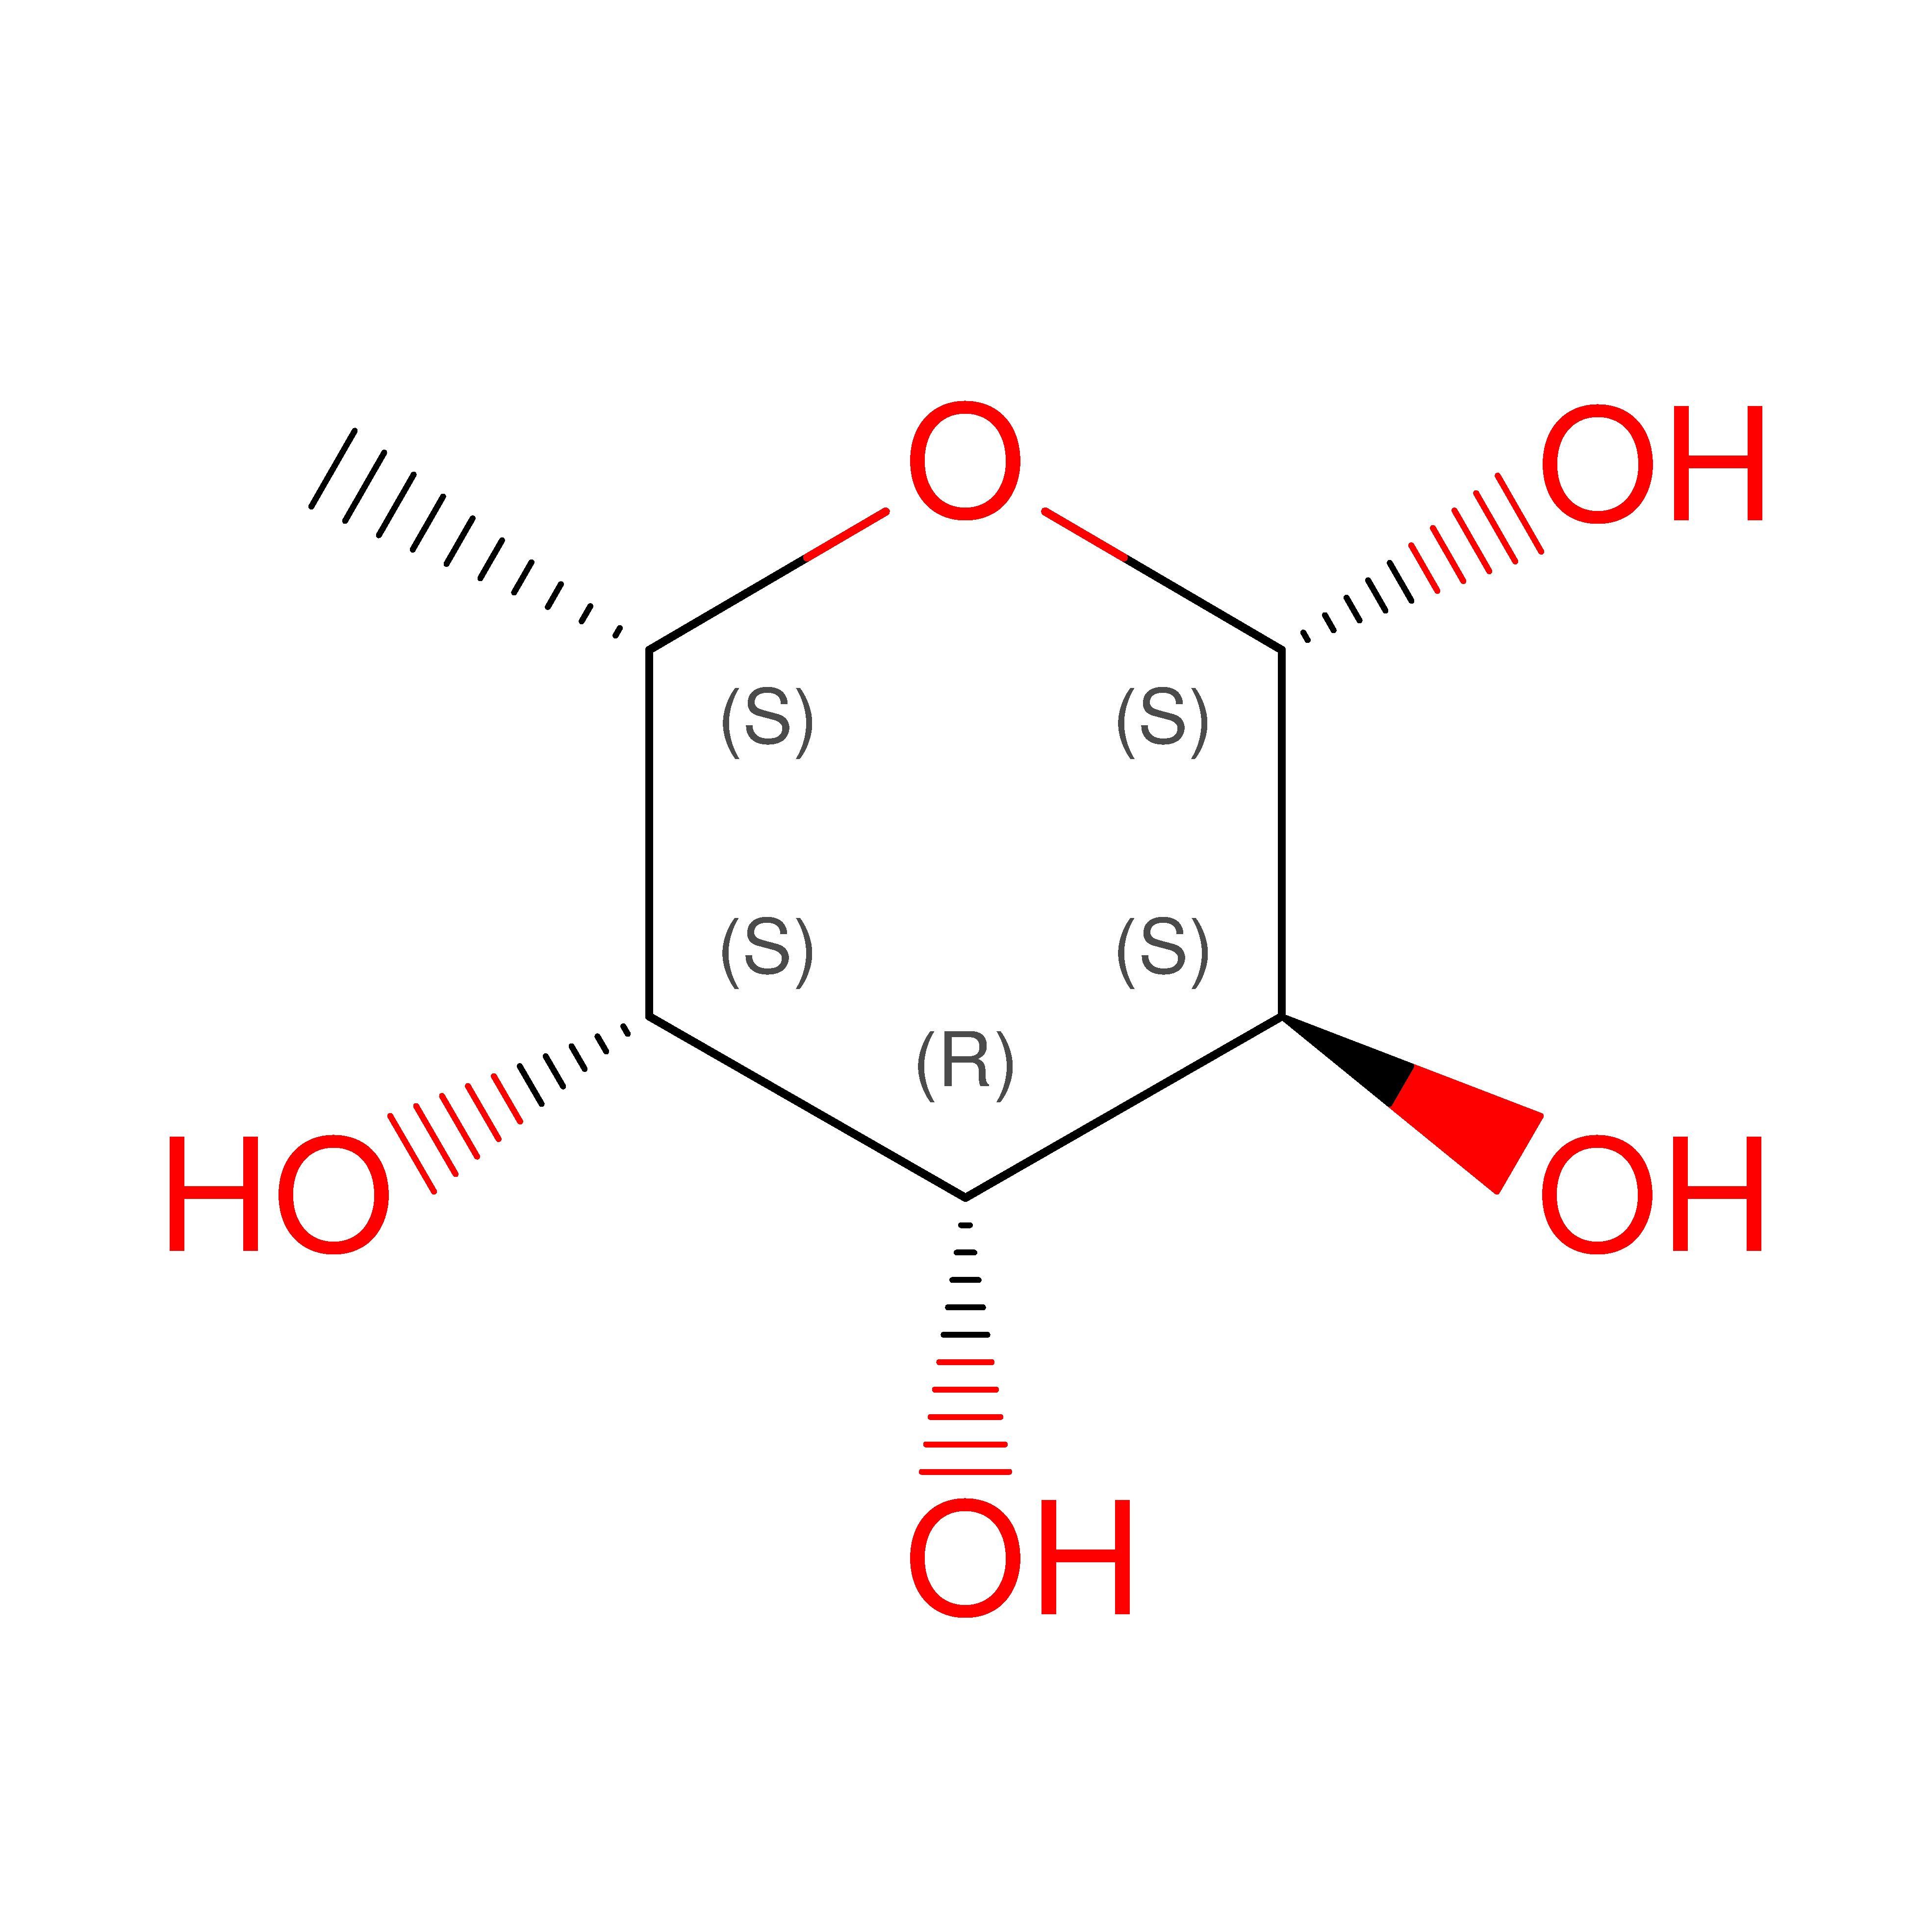
\psfig{file=figures/results/ligands/FUL.eps, width=1\textwidth}
        \end{subfigure}
      \end{figure}

      The main interactions for this protein-carbohydrates complex are the hydrogen bonds formed in its binding pockets \cite{hbonds_2023}. Effectively, the hydrogen bond potentials visualization agrees with the specific hydrogen bonds previously reported (figure \ref{fig:benchmark/1ofz}).

      Furthermore, most of the pocket is hydrophilic, which makes sense for a carbohydrate ligand, and the pocket is completely electropositive. Although there are some regions of potential, the stacking interactions are irrelevant for this ligand (figure \ref{fig:appx_benchmark/1ofz}).

      \begin{figure}[H]
        \centering
        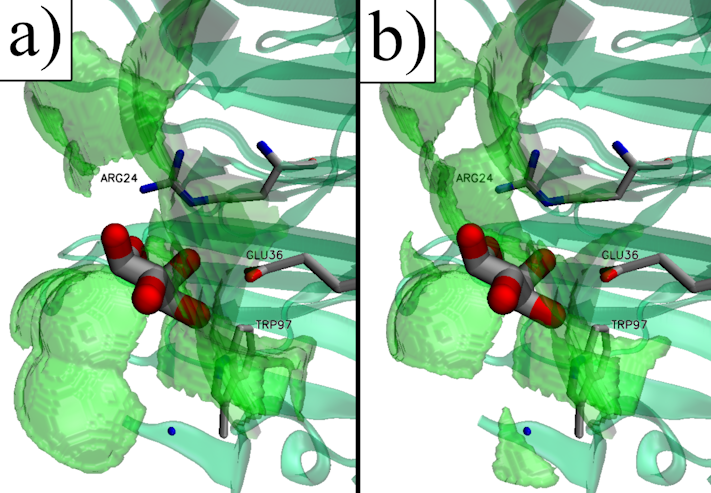
\includegraphics[width=0.7\textwidth]{figures/results/benchmark_prot/1ofz.png}
        \caption{\label{fig:benchmark/1ofz} Physical properties of the pocket for the protein system PDB:1OFZ. Potentials displayed: a) hydrogen bond acceptors, b) hydrogen bond donors.}
      \end{figure}
    \pagebreak

    \subsubsection{3DD0: Carbonic anhydrase II bound to 6-ethoxy-1,3-benzothiazole-2-sulfonamide}
      \begin{figure}[H] \centering
        \begin{subfigure}[c]{0.3\textwidth} \centering
          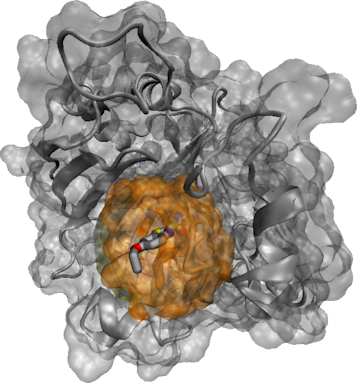
\includegraphics[width=1\textwidth]{figures/results/ps_prot/3dd0.png}
        \end{subfigure}
        \begin{subfigure}[c]{0.3\textwidth} \centering
          \psfig{file=figures/results/ligands/EZL.eps, width=1\textwidth}
        \end{subfigure}
      \end{figure}

      Similar to PDB:1EBY, the binding affinity reported for this system is mostly given by a couple of hydrogen bonds and several hydrophobic interactions \cite{benchmark_strong_2021}. The previously reported hydrophobic interactions match the potentials in figure \ref{fig:benchmark/3dd0}.

      Additionally, the expected hydrogen bonds also correspond to the visualization of their respective potentials. However, the stacking potential does not overlap with the aromatic section of the ligand. Finally, the pocket is mostly electronegative, with the exception of some positive charges (figure \ref{fig:appx_benchmark/3dd0}).

      \begin{figure}[H]
        \centering
        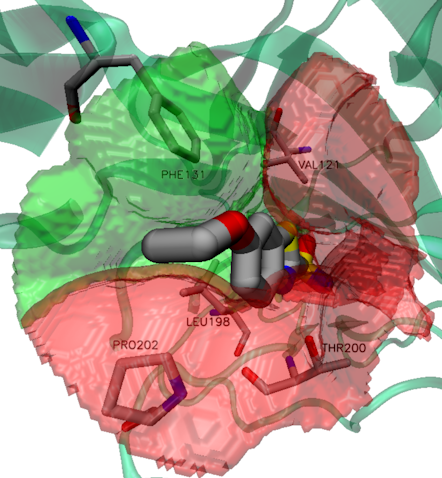
\includegraphics[width=0.5\textwidth]{figures/results/benchmark_prot/3dd0.png}
        \caption{\label{fig:benchmark/3dd0} Hydrophobic potential of the pocket for the protein system PDB:3DD0.}
      \end{figure}
    \pagebreak

    \subsubsection{3EE4: Mn/Fe oxidase bound to myristic acid}
      \begin{figure}[H] \centering
        \begin{subfigure}[c]{0.3\textwidth} \centering
          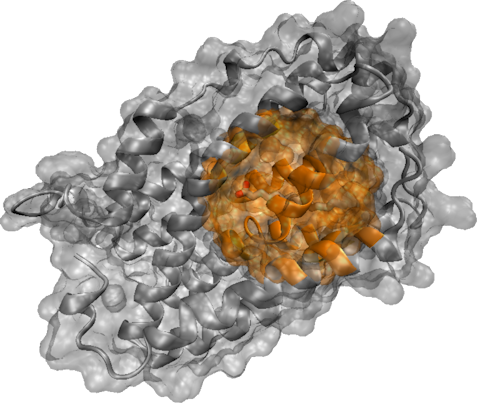
\includegraphics[width=1\textwidth]{figures/results/ps_prot/3ee4.png}
        \end{subfigure}
        \begin{subfigure}[c]{0.3\textwidth} \centering
          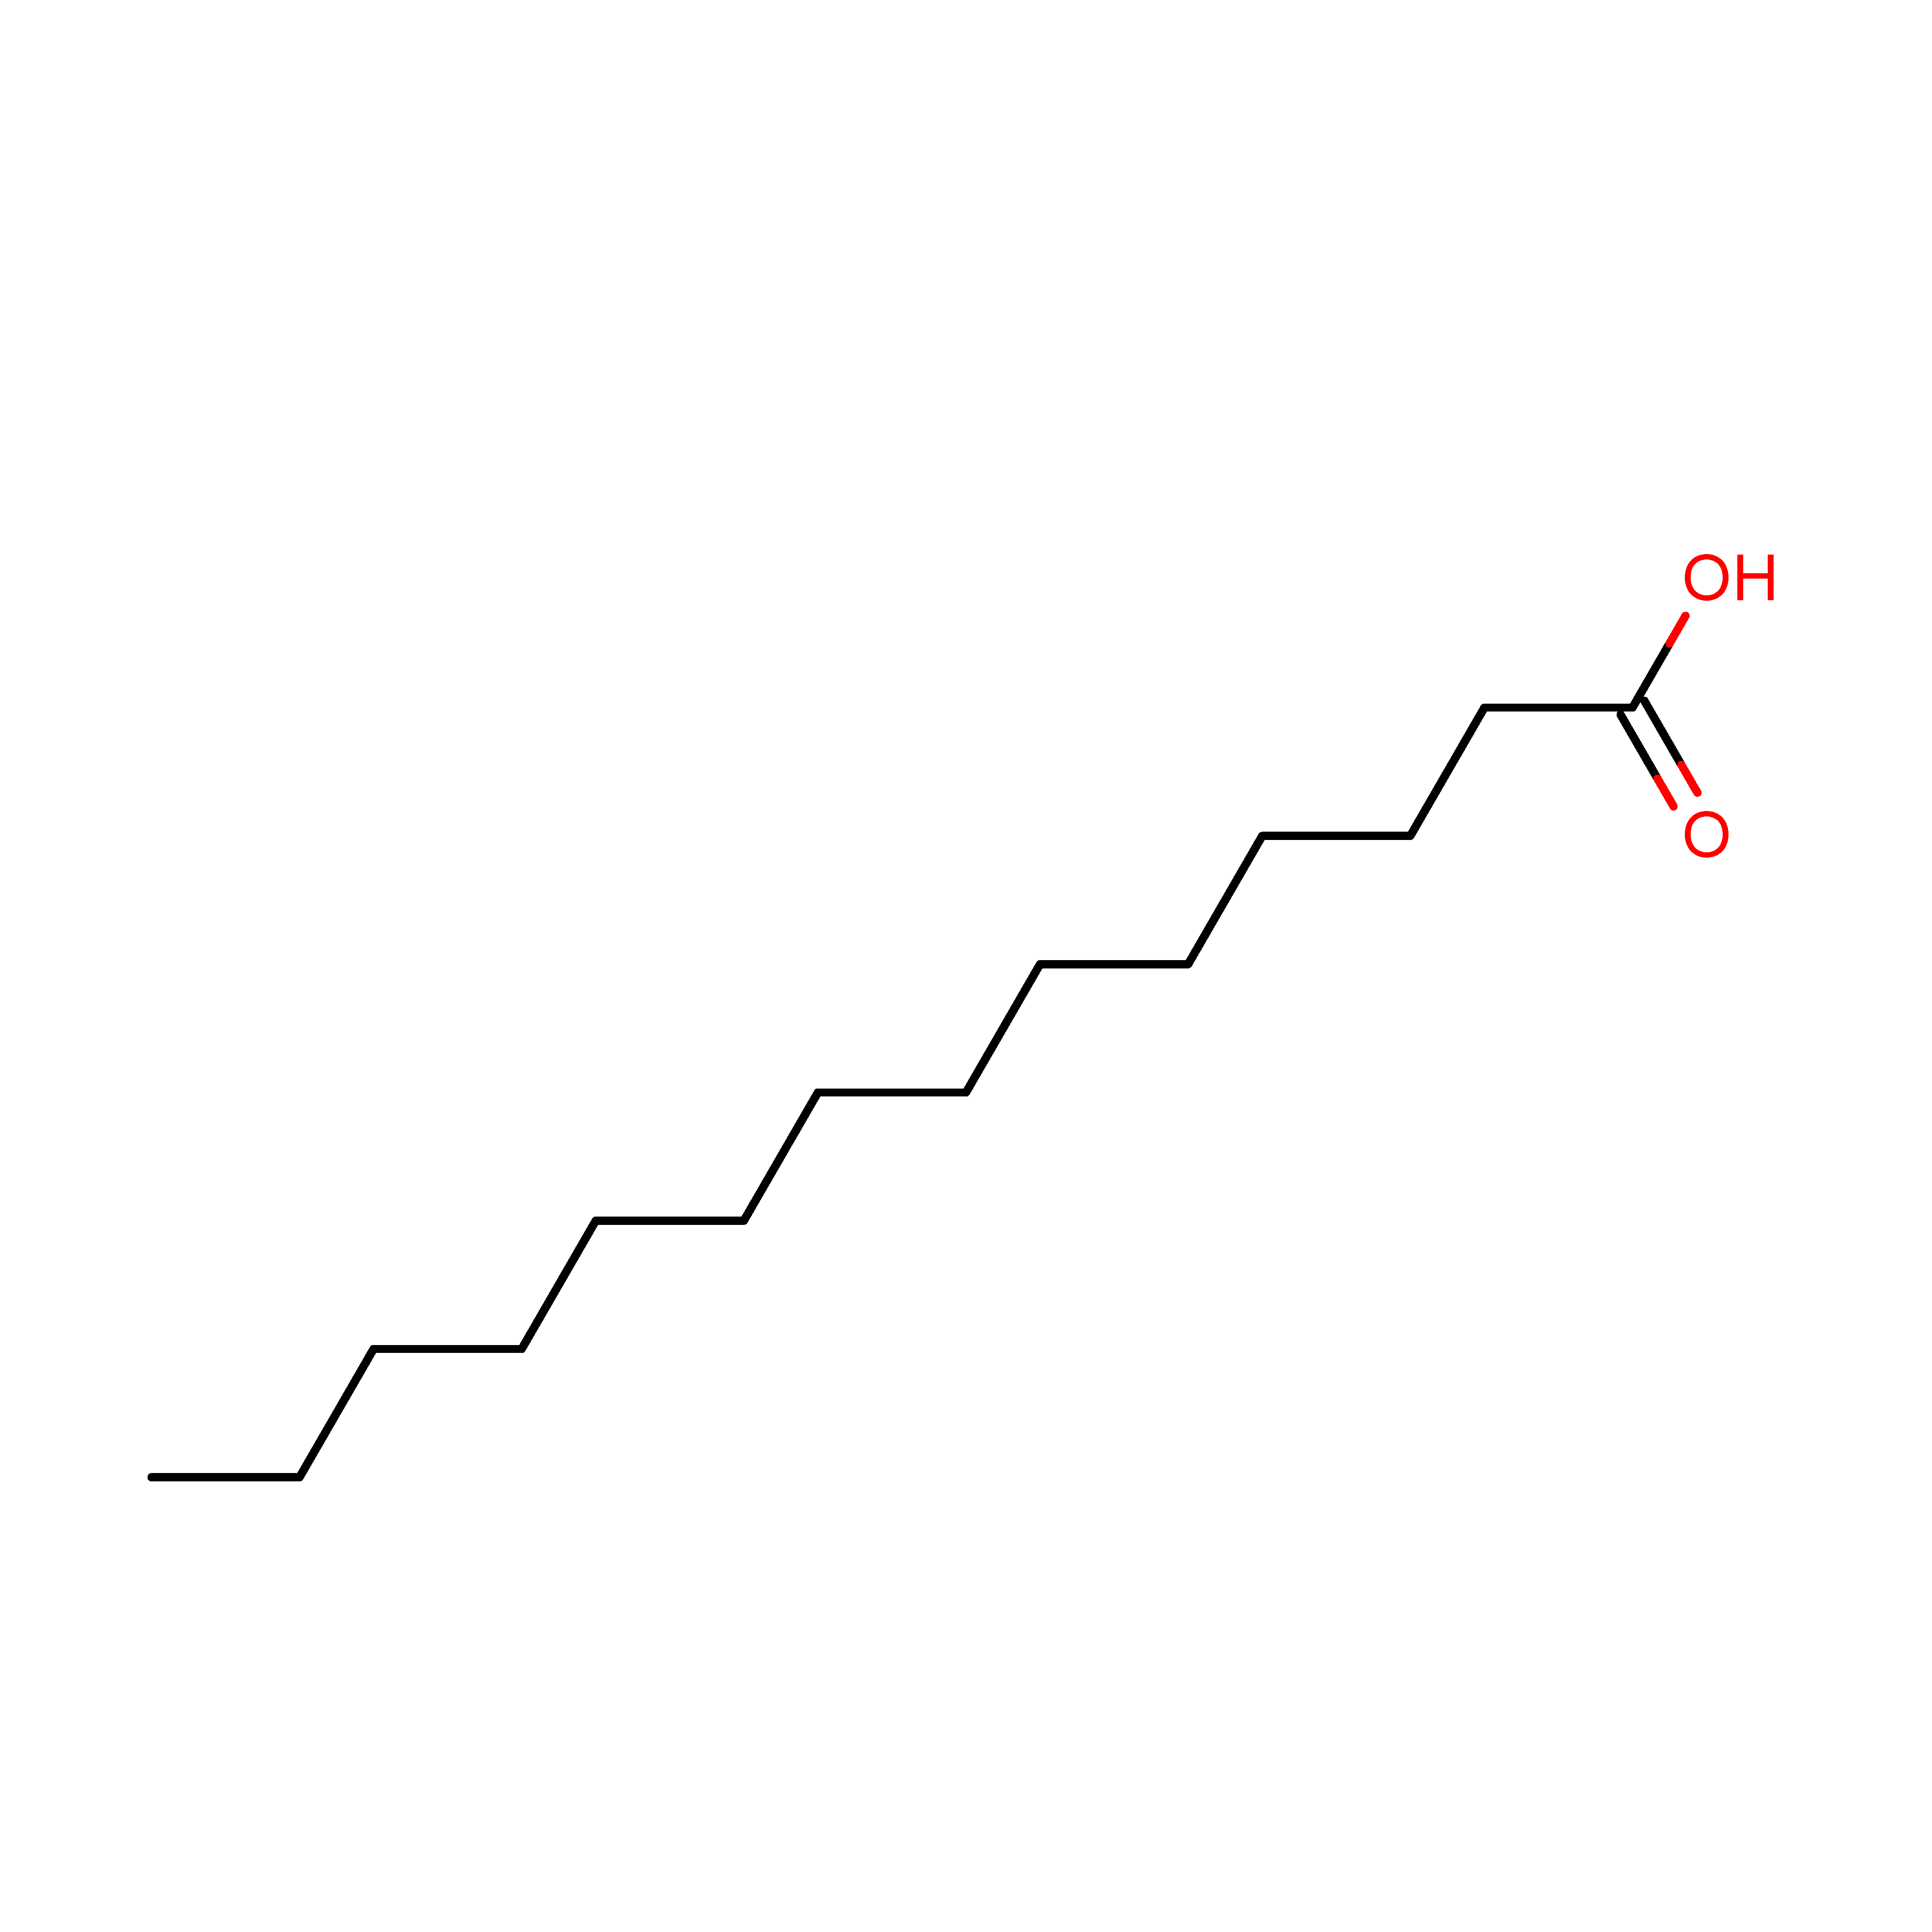
\psfig{file=figures/results/ligands/MYR.eps, width=1\textwidth}
        \end{subfigure}
      \end{figure}

      The pocket for this system has been described as a narrow and hydrophobic cavity that widens at its internal end, leading to a larger volume where metal cations coordinate with the protein and with more H-bond possibilities \cite{benchmark_hydrophobic_2009}. The representation of the hydrophobic potential matches accurately with this description, as seen in figure \ref{fig:benchmark/3ee4}. The aliphatic section of the ligand effectively overlaps with the mostly hydrophobic pocket, while the oxygen atoms at its extreme are placed in a hydrophilic region.

      Moreover, these oxygens also overlap with a region of hydrogen bond acceptancy, which is absent for the donors potential. The pocket is mostly electronegative, congruent with the presence of cations at the aforementioned hydrophilic region. Once more, some stacking potential is present but is not relevant for this ligand (figure \ref{fig:appx_benchmark/3ee4}).

      \begin{figure}[H]
        \centering
        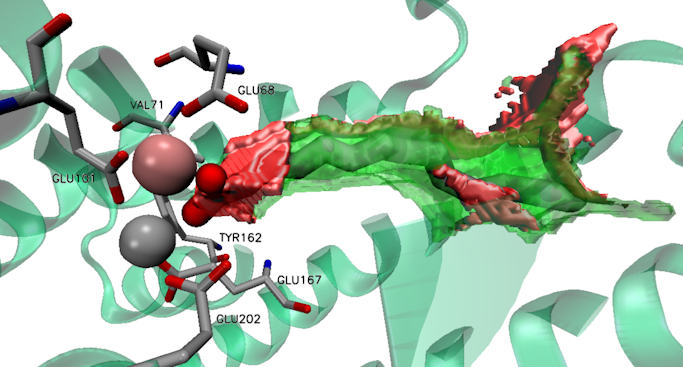
\includegraphics[width=0.8\textwidth]{figures/results/benchmark_prot/3ee4.png}
        \caption{\label{fig:benchmark/3ee4} Hydrophobic potential of the pocket for the protein system PDB:3EE4.}
      \end{figure}
    \pagebreak

    \subsubsection{5M9W: Thermolysin in complex with inhibitor JC65}
      \begin{figure}[H] \centering
        \begin{subfigure}[c]{0.3\textwidth} \centering
          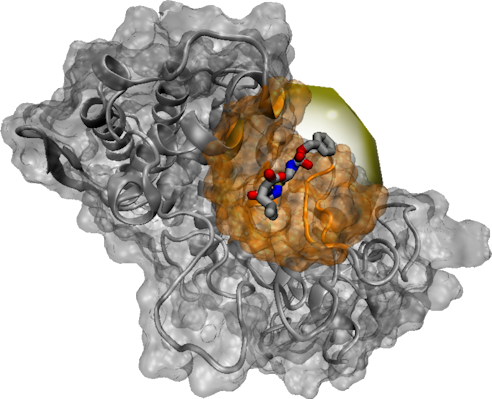
\includegraphics[width=1\textwidth]{figures/results/ps_prot/5m9w.png}
        \end{subfigure}
        \begin{subfigure}[c]{0.3\textwidth} \centering
          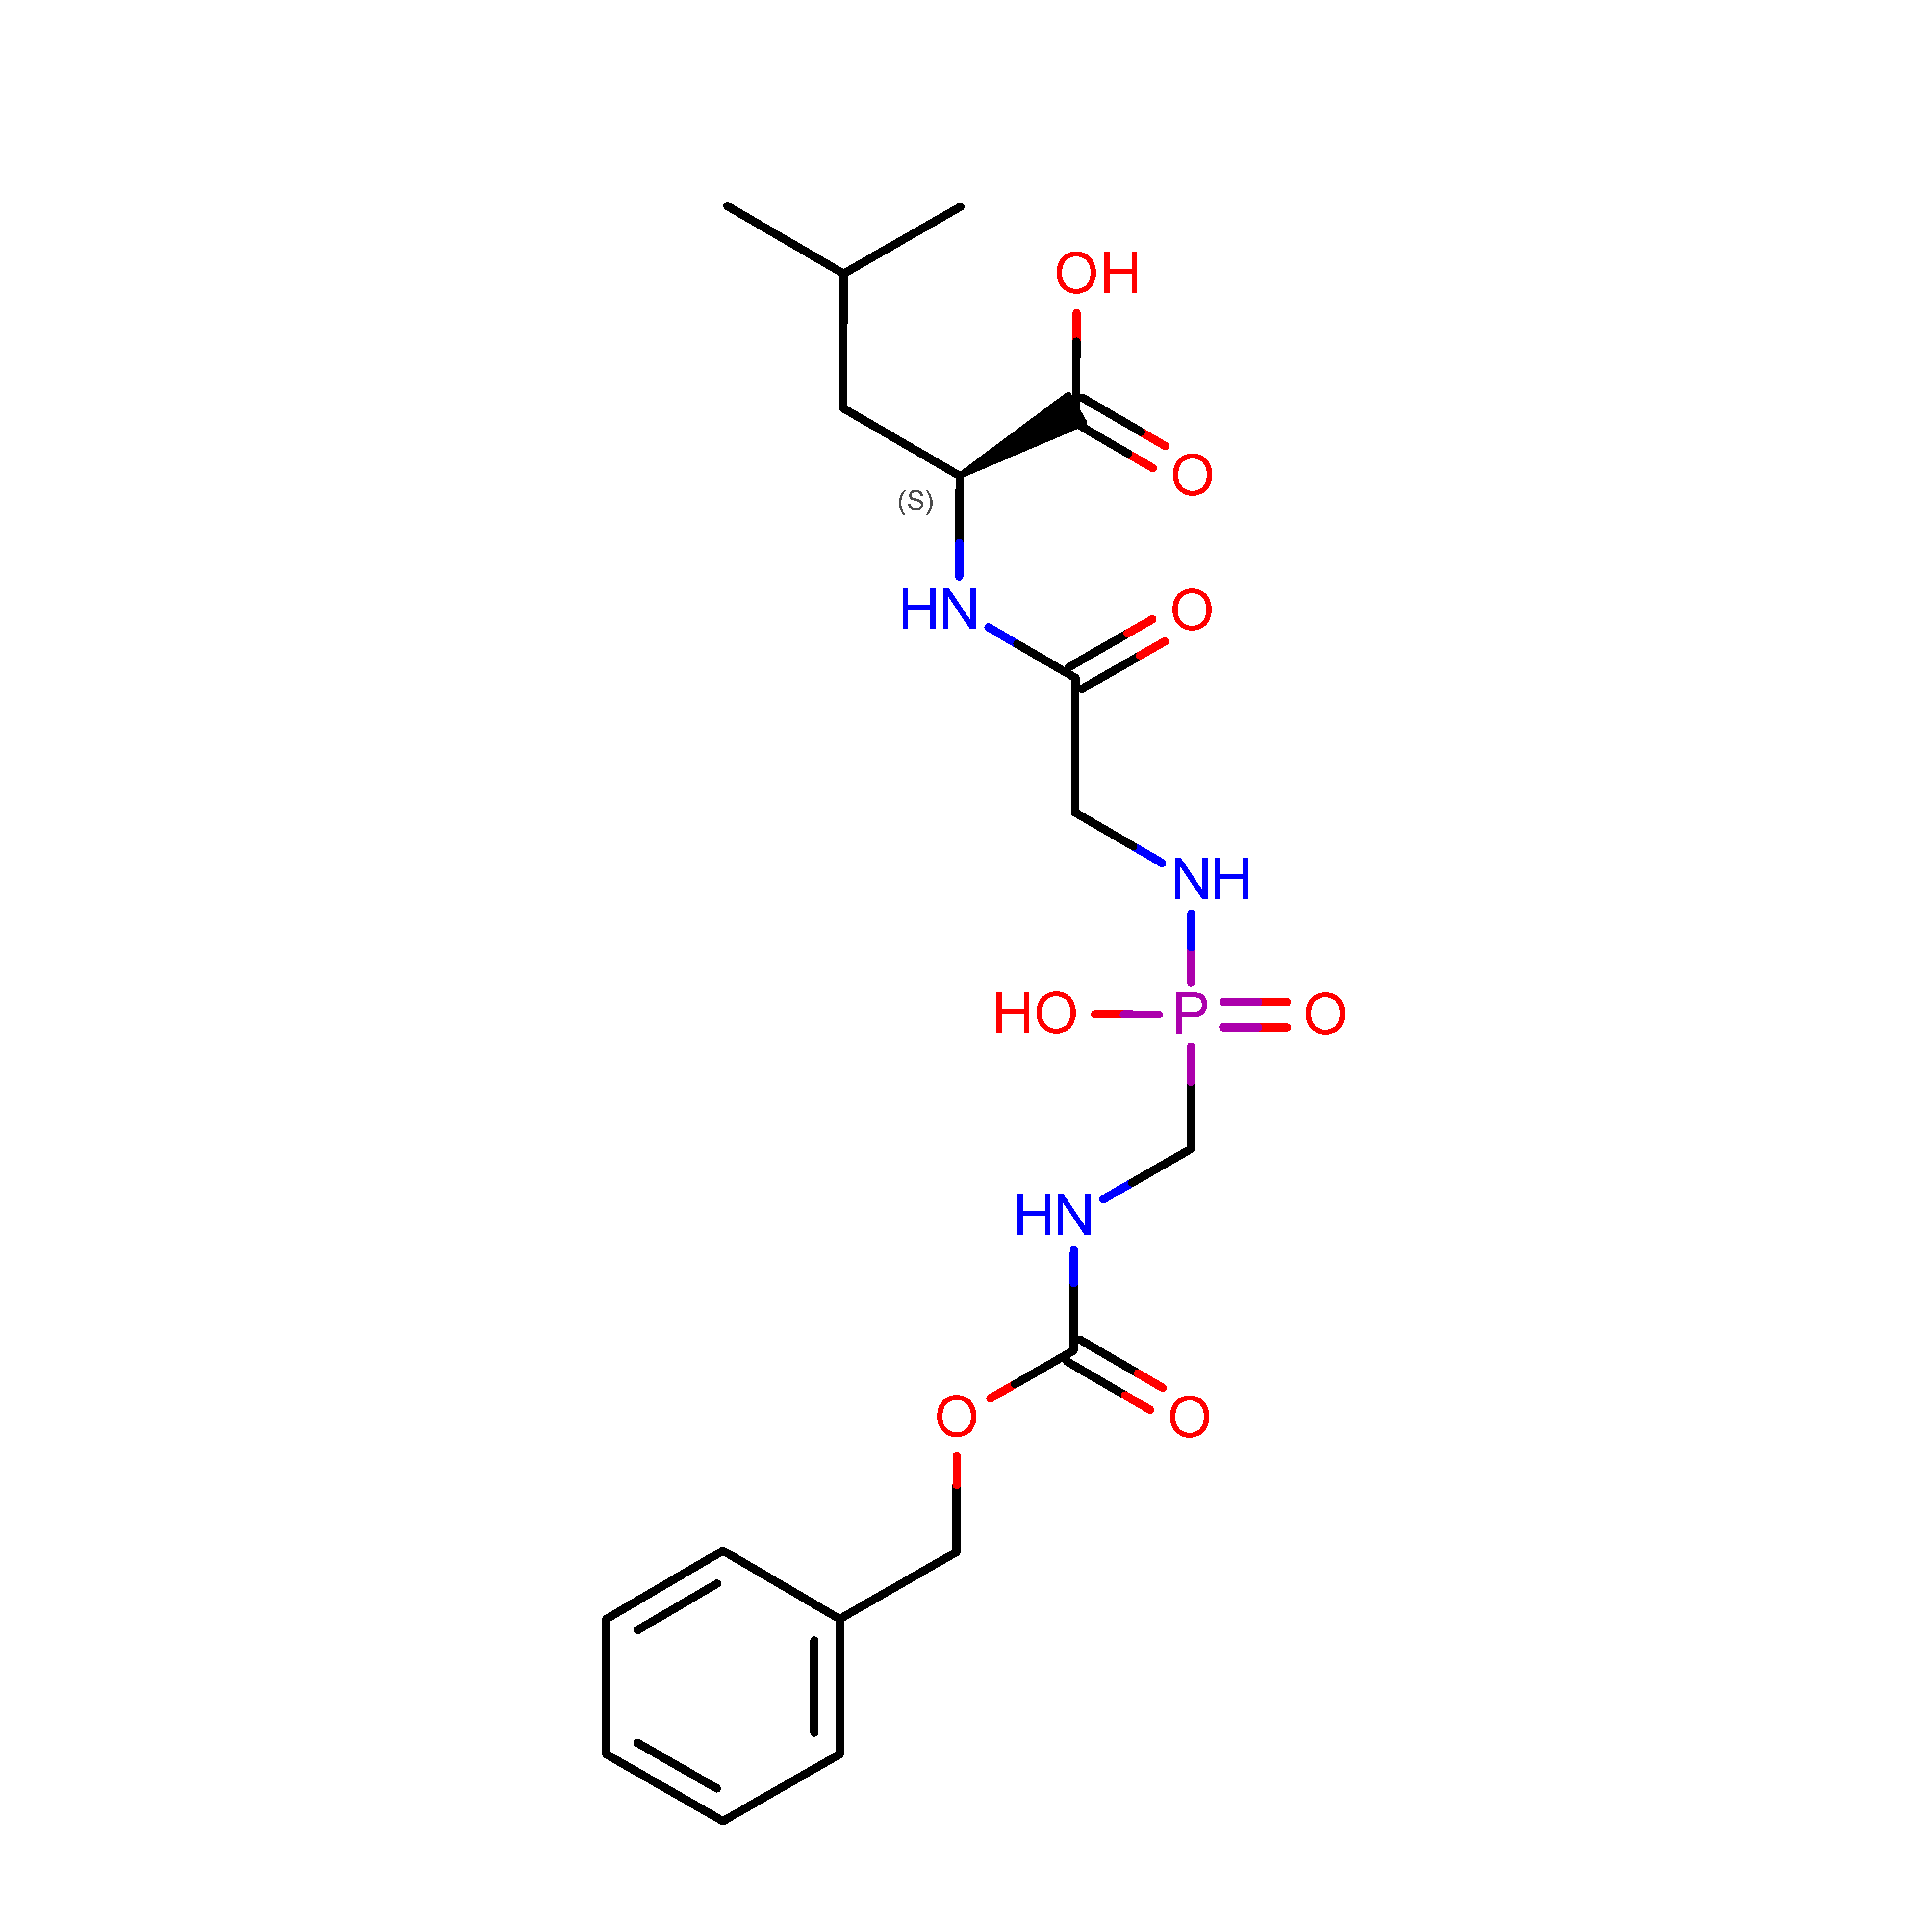
\psfig{file=figures/results/ligands/7GR.eps, width=1\textwidth}
        \end{subfigure}
      \end{figure}

      Hydrophobicity and hydrogen bonds play a major role in this system's binding pocket, as reported by \cite{hydrophobic_2017}. The potentials visualization shows the presence of mostly hydrophilic potential regions. Nevertheless, the hydrophobic groups of the ligand do match the hydrophobic regions described by the representation (figure \ref{fig:benchmark/5m9w}).

      Hydrogen bonds described in \cite{hydrophobic_2017} can also be inferred by observing the hydrogen bonds potentials of the system. Furthermore, the aromatic group of the ligand slightly overlaps with a large region of stacking potential. The pocket is mostly electronegative with some positive charges present (figure \ref{fig:appx_benchmark/5m9w}).

      \begin{figure}[H]
        \centering
        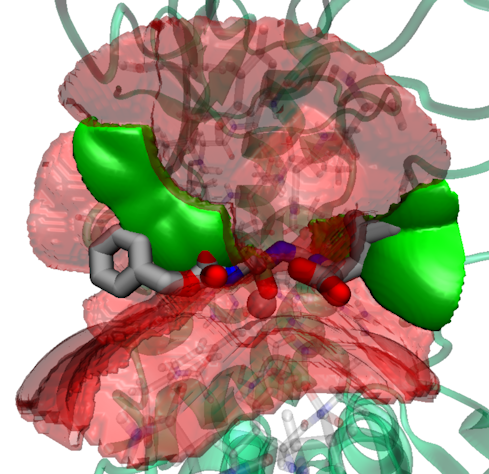
\includegraphics[width=0.5\textwidth]{figures/results/benchmark_prot/5m9w.png}
        \caption{\label{fig:benchmark/5m9w} Hydrophobic potential of the pocket for the protein system PDB:5M9W.}
      \end{figure}
    \pagebreak

    \subsubsection{6E9A: HIV-1 wild type protease bound to PDB:J0S}
      \begin{figure}[H] \centering
        \begin{subfigure}[c]{0.3\textwidth} \centering
          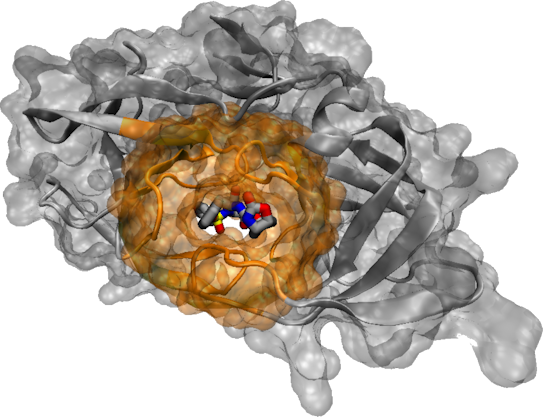
\includegraphics[width=1\textwidth]{figures/results/ps_prot/6e9a.png}
        \end{subfigure}
        \begin{subfigure}[c]{0.3\textwidth} \centering
          \psfig{file=figures/results/ligands/J0S.eps, width=1\textwidth}
        \end{subfigure}
      \end{figure}

      The pocket for this protein is reported to have a high binding affinity, which can be once again attributed to the presence of multiple hydrogen bonds and hydrophobic interactions \cite{benchmark_6e9a_2018}. The hydrogen bonds potentials visualized in figure \ref{fig:benchmark/6e9a} overlap with the expected heteroatoms for this interaction. The hydrophobic and hydrophilic regions also seem to coincide in some measure with their counterparts in the ligand, althought it is difficult to discern it correctly from the representations.

      As additional observations, the pocket has only two stacking potential regions, which do not coincide with the aromatic groups of its ligand. Moreover, the ligand is located in an electronegative region, while positive charges are more prevalent towards the extremes of the pocket (figure \ref{fig:appx_benchmark/6e9a}).

      \begin{figure}[H]
        \centering
        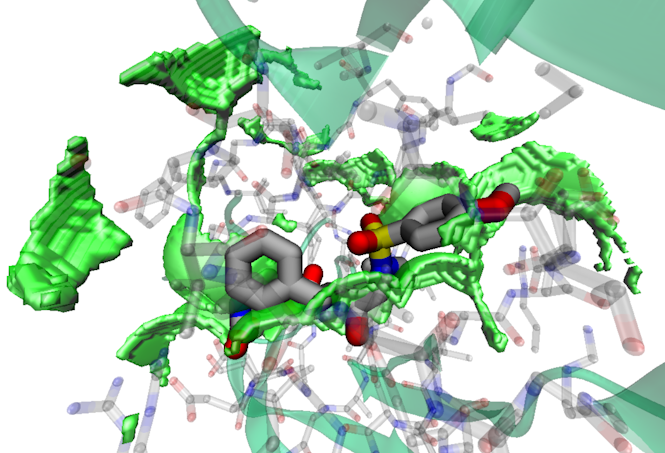
\includegraphics[width=0.7\textwidth]{figures/results/benchmark_prot/6e9a.png}
        \caption{\label{fig:benchmark/6e9a} Hydrogen bond acceptors potential of the pocket for the protein system PDB:6E9A.}
      \end{figure}
    \pagebreak

  \subsection{RNA Systems}
    \subsubsection{1AKX: HIV-2 trans activating region RNA in complex with argininamide}
      \textbf{Relevant ligand atoms for H-bond interactions (according to PLIP):} 975, 976 as acceptors; 969 as donor.

      \begin{figure}[H] \centering
        \begin{subfigure}[c]{0.3\textwidth} \centering
          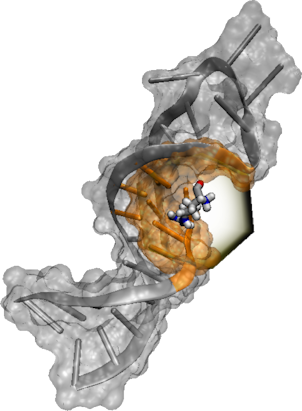
\includegraphics[width=1\textwidth]{figures/results/ps_rna/1akx.png}
        \end{subfigure}
        \begin{subfigure}[c]{0.3\textwidth} \centering
          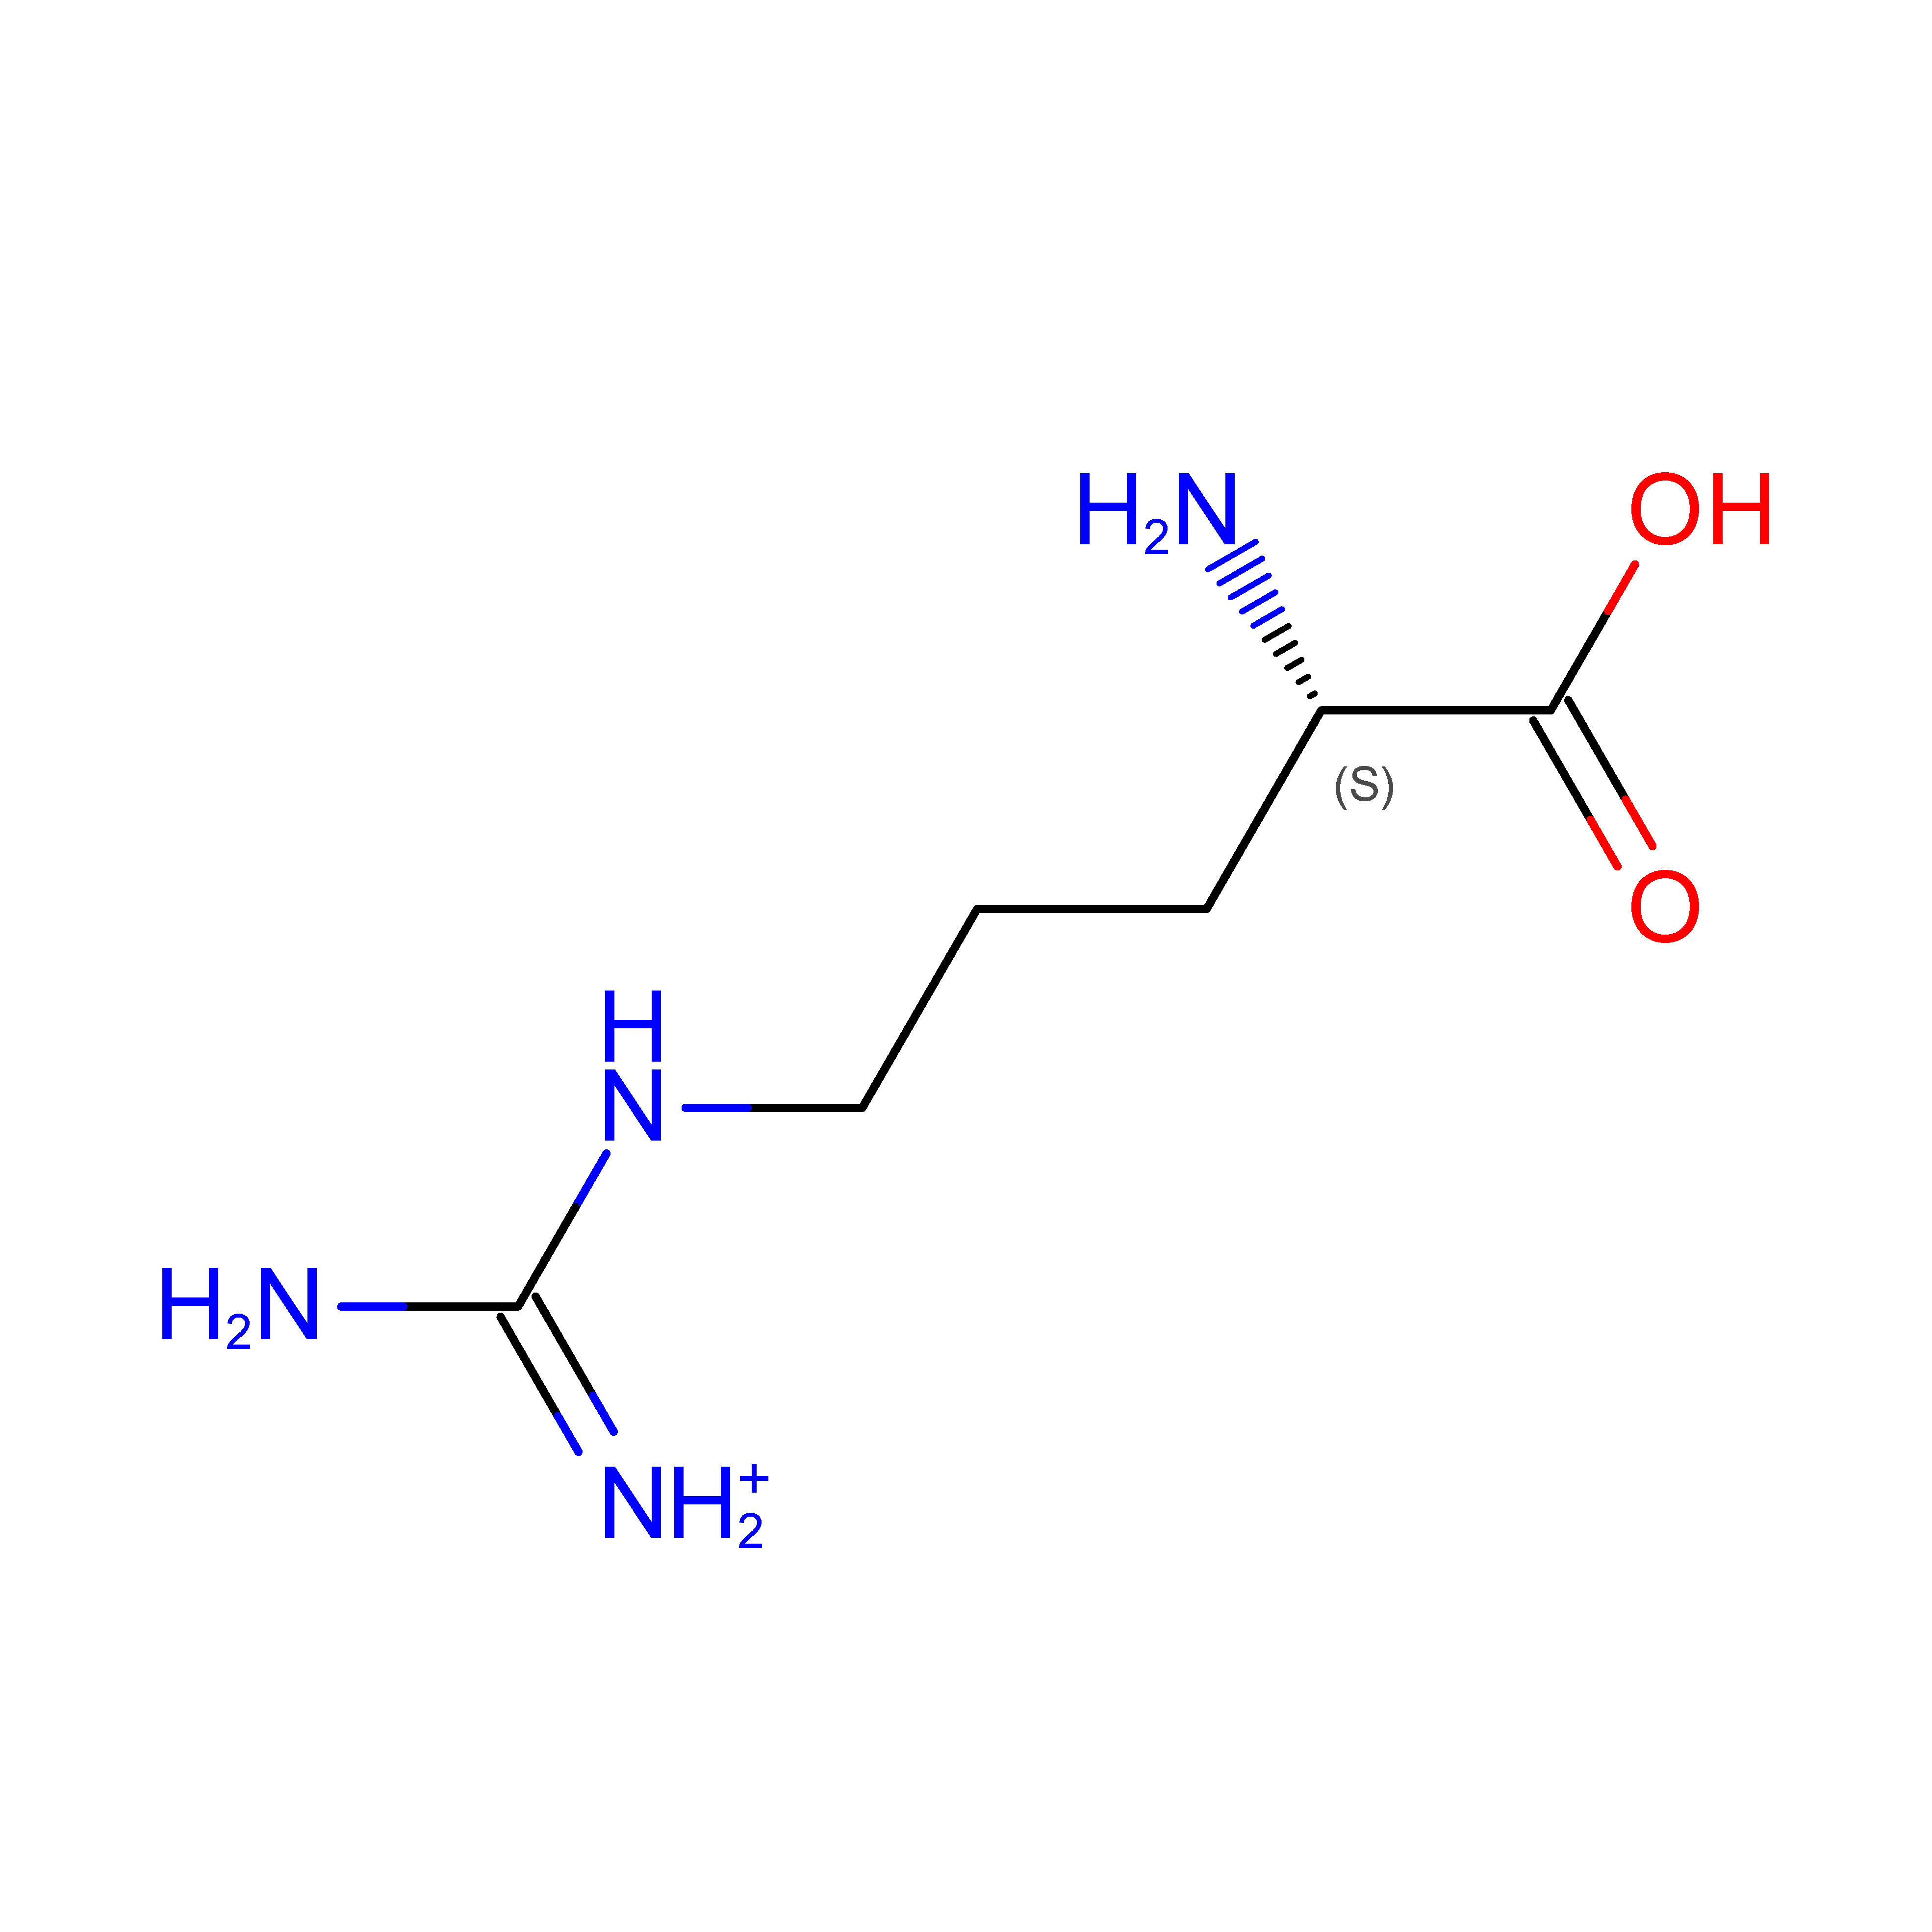
\psfig{file=figures/results/ligands/ARG.eps, width=1\textwidth}
        \end{subfigure}
      \end{figure}

      For this first system, the relevant ligand atom NH1 (index 975) enters in a small region of hydrogen bond acceptancy, while NH2 (index 976) does not (figure \ref{fig:benchmark/1akx}). On the other hand, the hydrogen bond donor potential does not overlap with the ligand at all, which does not correspond to the interaction suggested by PLIP. Finally, some stacking potential is present for this system, but irrelevant for the ligand of interest (figure \ref{fig:appx_benchmark/1akx}).

      \begin{figure}[H]
        \centering
        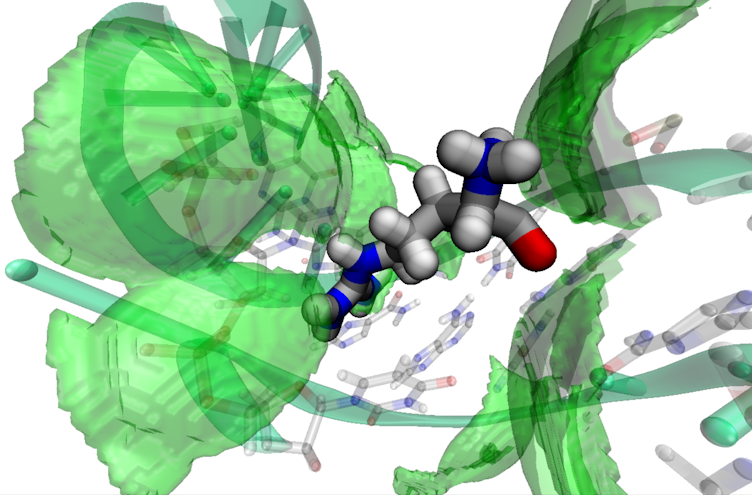
\includegraphics[width=0.6\textwidth]{figures/results/benchmark_rna/1akx.png}
        \caption{\label{fig:benchmark/1akx} Hydrogen bond acceptor potential for the RNA system PDB:1AKX.}
      \end{figure}
    \pagebreak

    \subsubsection{1I9V: Phenylalanine transfer RNA bound to neomycin}
      \textbf{Relevant ligand atoms for H-bond interactions (according to PLIP):} 1645, 1651, 1667, 1672, 1674 as acceptors; 1645 as donor.

      \begin{figure}[H] \centering
        \begin{subfigure}[c]{0.3\textwidth} \centering
          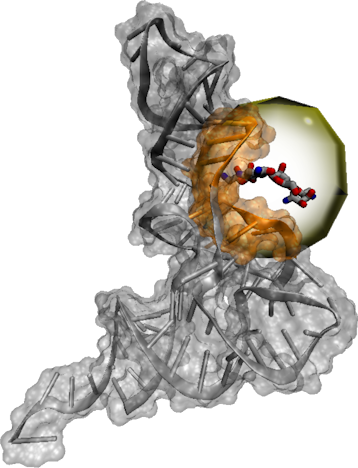
\includegraphics[width=1\textwidth]{figures/results/ps_rna/1i9v.png}
        \end{subfigure}
        \begin{subfigure}[c]{0.3\textwidth} \centering
          \psfig{file=figures/results/ligands/NMY.eps, width=1\textwidth}
        \end{subfigure}
      \end{figure}

      For the system presented in figure \ref{fig:benchmark/1i9v}, atoms N7, N9 and N6 (indices 1645, 1651 and 1667 respectively) fit nicely inside in regions of high hydrogen bond acceptancy. Atom N23 (index 1674) overlaps slightly, while O12 (index 1672) is close to overlapping but does not. However, similarly to the previous case, the predicted hydrogen bond donor interactions can not be inferred from the representation. Stacking potential is once again present but not relevant for this ligand (figure \ref{fig:appx_benchmark/1i9v}).

      \begin{figure}[H]
        \centering
        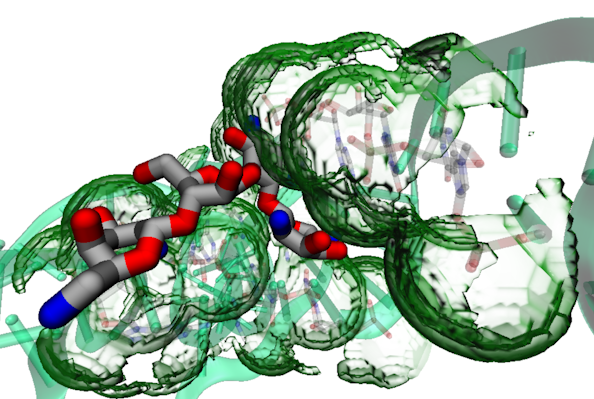
\includegraphics[width=0.6\textwidth]{figures/results/benchmark_rna/1i9v.png}
        \caption{\label{fig:benchmark/1i9v} Hydrogen bond acceptor potential for the RNA system PDB:1I9V.}
      \end{figure}
    \pagebreak

    \subsubsection{2ESJ: Complex between Lividomycin A and the 16S-Rrna A Site}
      \textbf{Relevant ligand atoms for H-bond interactions (according to PLIP):} 911, 913, 915, 920, 929, 935, 948 as acceptors; 909, 913, 924, 935 as donors.

      \begin{figure}[H] \centering
        \begin{subfigure}[c]{0.3\textwidth} \centering
          \includegraphics[width=1\textwidth]{figures/results/ps_rna/2esj.png}
        \end{subfigure}
        \begin{subfigure}[c]{0.3\textwidth} \centering
          \psfig{file=figures/results/ligands/LIV.eps, width=1\textwidth}
        \end{subfigure}
      \end{figure}

      All relevant atoms for the hydrogen bond acceptor potential overlap with the isosurface representation, altough atoms O62 and N32 (indices 915 and 920) are slightly offset (figure \ref{fig:benchmark/2esj}). In the case of hydrogen bond donor potential, atoms O51 and O23 (indices 909 and 924) overlap nicely with it, while N12 and N24 (indices 913 and 935) do not. Stacking potential is present but not relevant for this ligand (figure \ref{fig:appx_benchmark/2esj}).

      \begin{figure}[H]
        \centering
        \includegraphics[width=0.5\textwidth]{figures/results/benchmark_rna/2esj.png}
        \caption{\label{fig:benchmark/2esj} Hydrogen bond acceptor potential for the RNA system PDB:2ESJ.}
      \end{figure}
    \pagebreak

    \subsubsection{4F8U: Bacterial ribosomal decoding site in complex with sisomicin (C2 form)}
      \textbf{Relevant ligand atoms for H-bond interactions (according to PLIP):} 944, 945, 946, 948, 949 as acceptors; 944, 945, 950, 952 as donors.

      \begin{figure}[H] \centering
        \begin{subfigure}[c]{0.3\textwidth} \centering
          \includegraphics[width=1\textwidth]{figures/results/ps_rna/4f8u.png}
        \end{subfigure}
        \begin{subfigure}[c]{0.3\textwidth} \centering
          \psfig{file=figures/results/ligands/SIS.eps, width=1\textwidth}
        \end{subfigure}
      \end{figure}

      All relevant atoms for hydrogen bond acceptor potential overlap with the isosurface representation (figure \ref{fig:benchmark/4f8u}). In the case of hydrogen bond donor potential, atoms O51 and O53 (indices 950 and 952) overlap nicely, while N32 and N33 (indices 944 and 945) do not. Stacking potential is present but not relevant for this ligand (figure \ref{fig:appx_benchmark/4f8u}).

      \begin{figure}[H]
        \centering
        \includegraphics[width=0.5\textwidth]{figures/results/benchmark_rna/4f8u.png}
        \caption{\label{fig:benchmark/4f8u} Hydrogen bond acceptor potential for the RNA system PDB:4F8U.}
      \end{figure}
    \pagebreak

    \subsubsection{5BJO: Corn RNA aptamer in complex with DFHO}
      \textbf{Relevant ligand atoms for H-bond interactions (according to PLIP):} 1580, 1596 as acceptors; 1590, 1595 as donors.

      \begin{figure}[H] \centering
        \begin{subfigure}[c]{0.3\textwidth} \centering
          \includegraphics[width=1\textwidth]{figures/results/ps_rna/5kx9.png}
        \end{subfigure}
        \begin{subfigure}[c]{0.3\textwidth} \centering
          \psfig{file=figures/results/ligands/747.eps, width=1\textwidth}
        \end{subfigure}
      \end{figure}

      The aromatic groups of the ligand overlap significantly with its stacking potential. Two copies of residue 12 (guanine) seem to perform parallel stacking on one ring (from opposite sides), while the other aromatic ring is involved in parallel stacking with two copies of residue 25 (guanine) and perpendicular stacking with one copy of residue 24 (adenine) T (figure \ref{fig:benchmark/5bjo}.a). Similarly, both O1 (index 1580) and O19 (index 1596) overlap nicely with the hydrogen bond acceptor potential, with the latter being slightly offset (figure \ref{fig:benchmark/5bjo}.b). Finally, both N13 and N18 (indices 1590 and 1595) present a good overlap with the hydrogen bond donor potential (figure \ref{fig:appx_benchmark/5bjo}). All of these interactions could explain why this system has one of the largest binding affinities reported in the Hariboss database.

      \begin{figure}[H]
        \centering
        \includegraphics[width=0.7\textwidth]{figures/results/benchmark_rna/5bjo.png}
        \caption{\label{fig:benchmark/5bjo} Physical properties of the pocket for the RNA system PDB:5BJO. Potentials displayed: a) stacking, b) hydrogen bond acceptors.}
      \end{figure}
    \pagebreak

    \subsubsection{5KX9: FMN Riboswitch bound to PDB:6YG}
      \textbf{Relevant ligand atoms for H-bond interactions (according to PLIP):} 2337 as donor.

      \begin{figure}[H] \centering
        \begin{subfigure}[c]{0.3\textwidth} \centering
          \includegraphics[width=1\textwidth]{figures/results/ps_rna/6tf3.png}
        \end{subfigure}
        \begin{subfigure}[c]{0.3\textwidth} \centering
          \psfig{file=figures/results/ligands/6YG.eps, width=1\textwidth}
        \end{subfigure}
      \end{figure}

      The three aromatic groups from the ligand overlap significantly with the stacking potential: residue 48 (adenine) performs parallel stacking and residue 49 (adenine) perpendicular stacking to one ring, residue 85 (adenine) parallel stacking to the next ring and residue 62 (guanine) parallel stacking to the last ring (figure \ref{fig:benchmark/5kx9}). Although multiple heteroatoms overlap with the hydrogen bond acceptor potential, no relevant atoms for this interaction were found by PLIP. On the other hand, the relevant atom O07 (index 2337) overlaps with a corner of the hydrogen bond donor potential region (figure \ref{fig:appx_benchmark/5kx9}).

      \begin{figure}[H]
        \centering
        \includegraphics[width=0.5\textwidth]{figures/results/benchmark_rna/5kx9.png}
        \caption{\label{fig:benchmark/5kx9} Stacking potential for the RNA system PDB:5KX9.}
      \end{figure}
    \pagebreak

    \subsubsection{6TF3: ADP-binding domain of the NAD+ riboswitch in complex with Cordycepin 5-triphosphate}
      \textbf{Relevant ligand atoms for H-bond interactions (according to PLIP):} 1135, 1145 as donors.

      \begin{figure}[H] \centering
        \begin{subfigure}[c]{0.3\textwidth} \centering
          \includegraphics[width=1\textwidth]{figures/results/ps_rna/7oax0.png}
        \end{subfigure}
        \begin{subfigure}[c]{0.3\textwidth} \centering
          \psfig{file=figures/results/ligands/3AT.eps, width=1\textwidth}
        \end{subfigure}
      \end{figure}

      Another example of a ligand's aromatic group overlapping precisely on the predicted stacking potential region can be seen in figure \ref{fig:benchmark/6tf3}.a. In this case, residue 8 (adenine) performs parallel stacking on the aromatic group, as denoted by the well defined potential torus. For the hydrogen bond donor potential, N3 (index 1145) has a good overlap, while O2' (index 1135) is close to the potential but does not quite overlap (figure \ref{fig:benchmark/6tf3}.b). The hydrogen bond acceptor potential is again present in the system but its respective interaction is not described by PLIP (figure \ref{fig:appx_benchmark/6tf3}).

      \begin{figure}[H]
        \centering
        \includegraphics[width=0.7\textwidth]{figures/results/benchmark_rna/6tf3.png}
        \caption{\label{fig:benchmark/6tf3} Physical properties of the pocket for the RNA system PDB:6TF3. Potentials displayed: a) stacking, b) hydrogen bond donors.}
      \end{figure}
    \pagebreak

    \subsubsection{7OAX: Chili RNA aptamer in complex with spermine}
      \textbf{Relevant ligand atoms for H-bond interactions (according to PLIP):} 4692, 4696, 4705 as acceptors; 4696 as donor.

      \begin{figure}[H] \centering
        \begin{subfigure}[c]{0.3\textwidth} \centering
          \includegraphics[width=1\textwidth]{figures/results/ps_rna/7oax1.png}
        \end{subfigure}
        \begin{subfigure}[c]{0.3\textwidth} \centering
          \psfig{file=figures/results/ligands/SPM.eps, width=1\textwidth}
        \end{subfigure}
      \end{figure}

      For this system, all relevant atoms overlap with the hydrogen bond acceptor potential (figure \ref{fig:benchmark/7oax0}). However the hydrogen bond donor potential regions do not overlap with the relevant atoms. Stacking potential is present but not relevant for this ligand (figure \ref{fig:appx_benchmark/7oax0}).

      \begin{figure}[H]
        \centering
        \includegraphics[width=0.5\textwidth]{figures/results/benchmark_rna/7oax0.png}
        \caption{\label{fig:benchmark/7oax0} Hydrogen bond acceptor potential for the RNA system PDB:7OAX (ligand: SPM).}
      \end{figure}
    \pagebreak

    \subsubsection{7OAX: Chili RNA aptamer in complex with DMHBO+}
      \textbf{Relevant ligand atoms for H-bond interactions (according to PLIP):} 4464 as acceptor; 4459, 4465 as donors.

      \begin{figure}[H] \centering
        \begin{subfigure}[c]{0.3\textwidth} \centering
          \includegraphics[width=1\textwidth]{figures/results/ps_rna/5bjo.png}
        \end{subfigure}
        \begin{subfigure}[c]{0.3\textwidth} \centering
          \psfig{file=figures/results/ligands/V5Z.eps, width=1\textwidth}
        \end{subfigure}
      \end{figure}

      The stacking potential becomes again relevant for this complex, with residues 14 and 31 (both guanines) performing parallel stacking to two of the ligand's aromatic rings (figure \ref{fig:benchmark/7oax1}.a). Both N08 and O25 (indices 4459 and 4465) overlap (although slighlty offset) with the hydrogen bond donor potential (figure \ref{fig:benchmark/7oax1}.b). The relevant atom O12 (index 4464) overlaps with a dense region of hydrogen bond acceptor potential (figure \ref{fig:appx_benchmark/7oax1}).

      \begin{figure}[H]
        \centering
        \includegraphics[width=0.8\textwidth]{figures/results/benchmark_rna/7oax1.png}
        \caption{\label{fig:benchmark/7oax1} Physical properties of the pocket for the RNA system PDB:7OAX (ligand: V5Z). Potentials displayed: a) stacking, b) hydrogen bond donors.}
      \end{figure}
    \pagebreak

    \subsubsection{8EYV: Beetroot dimer bound to DFHO}
      \textbf{Relevant ligand atoms for H-bond interactions (according to PLIP):} 1993, 1998 as donors.

      \begin{figure}[H] \centering
        \begin{subfigure}[c]{0.3\textwidth} \centering
          \includegraphics[width=1\textwidth]{figures/results/ps_rna/8eyv.png}
        \end{subfigure}
        \begin{subfigure}[c]{0.3\textwidth} \centering
          \psfig{file=figures/results/ligands/747.eps, width=1\textwidth}
        \end{subfigure}
      \end{figure}

      The last RNA benchmark also presents a relevant stacking interaction, revealed both by PLIP and the potential visualization: residues 16 (adenine) and 17 (guanine) perform parallel stacking to one aromatic ring of the ligand, while residue 38 (uracyl) performs to the other ring (figure \ref{fig:benchmark/8eyv}.a). furthermore, both N13 and N18 (indices 1993 and 1998) overlap nicely with the hydrogen bond donor potential (figure \ref{fig:benchmark/8eyv}.b). The hydrogen bond acceptor potential is present in the system but its respective interaction is not described by PLIP (figure \ref{fig:appx_benchmark/8eyv}).

      \begin{figure}[H]
        \centering
        \includegraphics[width=0.7\textwidth]{figures/results/benchmark_rna/8eyv.png}
        \caption{\label{fig:benchmark/8eyv} Physical properties of the pocket for the RNA system PDB:8EYV. Potentials displayed: a) stacking, b) hydrogen bond donors.}
      \end{figure}
    \pagebreak


%%%%%%%%%%%%%%%%%%%%%%%%%%%%%%%%%%%%%%%%%%%%%%%%%%%%%%%%%%%%%%%%%%%%%%%%%%%%%%%%
